\documentclass[usenames,dvipsnames,svgnames,table]{beamer}

\usetheme{AnnArbor}
\usepackage{lmodern}
\usepackage{amsmath}
\usepackage{enumitem}
\usepackage{multicol}
\usepackage{graphicx}
\usepackage{epstopdf}
\usepackage{pgffor}
\usepackage{rotating}

\newcommand{\experiment}[1]{\textcolor{blue}{#1}}
\newcommand{\CMS}[1]{\experiment{#1}}
\newcommand{\ATLAS}[1]{\experiment{#1}}
\newcommand{\theory}[1]{\textcolor{red}{#1}}
\newcommand{\dontknow}[1]{\textcolor{cyan}{#1}}
\newcommand{\me}[1]{\textbf{\CMS{#1}}}

\newcommand{\spin}[1]{\text{spin }#1}
\renewcommand{\therefore}{\Rightarrow}

\newenvironment{variableblock}[3]{
%http://tex.stackexchange.com/questions/33231/how-to-change-the-color-of-a-block-within-a-custom-beamer-sty-theme-file
  \setbeamercolor{block body}{#2}
  \setbeamercolor{block title}{#3}
  \begin{block}{#1}\end{block}}

\title[JHUGen and MELA]{Tools for the Higgs boson CP studies: \\ JHUGen and MELA}

\author[Heshy Roskes]{\CMS{I. Anderson}, \CMS{S. Bolognesi}, \theory{F. Caola}, \ATLAS{Y. Gao}, \CMS{A. Gritsan}, \CMS{Z. Guo}, \CMS{C. Martin}, \theory{K. Melnikov}, \me{H. Roskes}, \CMS{U. Sarica}, \theory{M. Schulze}, \CMS{N. Tran}, \CMS{A. Whitbeck}, \CMS{M. Xiao}, \CMS{C. You}, \theory{Y. Zhou}
\texorpdfstring{\\ \leavevmode
\\
\theory{Theory}, \experiment{experiment}}{}}

\date{August 4, 2015}

%\author{I. Anderson, S. Bolognesi, F. Caola, Y. Gao, A. Gritsan, C. Martin, Z. Guo, K. Melnikov, {H. Roskes}, U. Sarica, M. Schulze, N. Tran, A. Whitbeck, M. Xiao, C. You, Y. Zhou}



\begin{document}

\begin{frame}
\titlepage
\end{frame}

\begin{frame}{Framework}

\begin{itemize}
\small
\item JHUGen
\begin{itemize}
\item Event generation
\end{itemize}
\item JHUGenMELA
\begin{itemize}
\item Discriminants for anomalous coupling fits and background suppression
\item Reweighting
\end{itemize}
\item AnalyticMELA
\begin{itemize}
\item Discriminants for anomalous coupling fits and background suppression
\item Analytic multidimensional fits
\item Validation
\end{itemize}
\end{itemize}

\end{frame}


\begin{frame}{JHU Generator}
\begin{itemize} \small
\begin{multicols}{2}
\item $gg\to H$
\item $gg/gq\to H+\text{jet}$
\item $gg/gq/q\bar{q}\to H+2\text{ jets}$ (QCD)
\item $q\bar{q}\to H+2\text{ jets}$ (VBF)
\item $q\bar{q}\to V^*\to V+H$ (VH)
\item $gg/q\bar{q}\to t\bar{t}H$
\begin{itemize}
\item $t\to Wb \to l\nu b/q\bar{q}^\prime b$
\end{itemize}
\item $q\bar{q}\to\spin{1}$
\item $gg/q\bar{q}\to\spin{2}$ \normalsize
\item %blank for alignment
\end{multicols}
\item
\item Decay:
\begin{itemize}[label={$\to$}] \small
\item \(ZZ^*+Z\gamma^*+\gamma^*\gamma^*\to \text{any combination of $l^+l^-$, $2\nu$, $q\bar{q}$}\)
\item \(W^+W^-\to \text{any combination of $l\nu$ and $q\bar{q}^\prime$}\)
\item $Z\gamma$, $\gamma\gamma$
\end{itemize}
\item Production and decay in one step for spin 1 and spin 2
\item \texttt{ReadLHE} mode for other processes or to decay events from other generators
\end{itemize}
\end{frame}

\begin{frame}{Parameterization}
\begin{itemize}
%\item Most general parameterization of anomalous couplings:
\item \small
$
A(HVV) \sim
$
\begin{itemize}
\item
$
\left[ a_{1}
+ \textcolor{Green}{\frac{q_{V_1}^2 +  q_{V_2}^{2}}{\left(\Lambda_{1} \right)^{2}}}
+ \textcolor{magenta}{\frac{(q_{V_1} + q_{V_2})^{2}}{\left(\Lambda_{Q} \right)^{2}}}
\right]
m_{V_1}^2 \epsilon_{V_1}^* \epsilon_{V_2}^*
+ \textcolor{red}{a_{2}  f_{\mu \nu}^{*(1)}f^{*(2),\mu\nu}}
+ \textcolor{blue}{a_{3}   f^{*(1)}_{\mu \nu} {\tilde f}^{*(2)\mu\nu}}
$
\end{itemize}
%\normalsize Lagrangian (equivalent)
\tiny
\item
$
 {L}(HVV) \sim
$
\begin{itemize}
\item
$
a^{ZZ}_{1}\frac{m_{Z}^2}{2} H Z^{\mu}Z_{\mu}
- \textcolor{Green}{\frac{1}{\left(\Lambda^{ZZ}_{1}\right)^{2}} m_{Z}^2 H  Z^{\mu} \Box Z_{\mu}}
- \textcolor{magenta}{\frac{1}{2\left(\Lambda^{ZZ}_{Q}\right)^{2}} m_{Z}^2 \Box H  Z^{\mu} Z_{\mu}}
- \textcolor{red}{\frac{1}{2}a^{ZZ}_{2} H  Z^{\mu\nu}Z_{\mu\nu}}
- \textcolor{blue}{\frac{1}{2}a^{ZZ}_{3} H  Z^{\mu\nu}{\tilde Z}_{\mu\nu}}
$
\item
$
+ a_{1}^{WW}{m_{W}^2} H W^{+\mu} W^{-}_{\mu}
- \textcolor{Green}{\frac{1}{\left(\Lambda_{1}^{WW}\right)^{2}} m_{W}^2 H
  \left(  W^{-}_{\mu} \Box W^{+\mu} + W^{+}_{\mu} \Box W^{-\mu} \right)}
$
\begin{itemize}
\item
$
- \textcolor{magenta}{\frac{1}{\left(\Lambda_{Q}\right)^{2}} m_{W}^2 \Box H  W^{+\mu} W^{-}_{\mu}}
- \textcolor{red}{a_{2}^{WW} H W^{+\mu\nu}W^{-}_{\mu\nu}}
- \textcolor{blue}{a_{3}^{WW} H W^{+\mu\nu}{\tilde W}^{-}_{\mu\nu}}
$
\end{itemize}
\item
$
+ \textcolor{Green}{\frac{1}{\left(\Lambda_{1}^{Z\gamma} \right)^{2}} m_{Z}^2 H  Z_\mu \partial_\nu F^{\mu\nu}}
- \textcolor{red}{a_{2}^{Z\gamma} H F^{\mu\nu} Z_{\mu\nu}}
- \textcolor{blue}{a_{3}^{Z\gamma} H  F^{\mu\nu}{\tilde Z}_{\mu\nu}}
$
\item
$
- \textcolor{red}{\frac{1}{2}a_{2}^{\gamma\gamma} H  F^{\mu\nu}F_{\mu\nu}}
- \textcolor{blue}{\frac{1}{2}a_{3}^{\gamma\gamma}H  F^{\mu\nu}{\tilde F}_{\mu\nu}}
$
\item
$
- \textcolor{red}{\frac{1}{2}a_{2}^{gg} H  G^{\mu\nu}_a G^a_{\mu\nu}}
- \textcolor{blue}{\frac{1}{2}a_{3}^{gg}H  G^{\mu\nu}_a{\tilde G}^a_{\mu\nu}}
$
\end{itemize}
\item \small Similar for spin 1 and spin 2
\item
\item Predictions are leading order QCD
\item POWHEG (NLO QCD) $gg\to H$ $\longrightarrow$ JHUGen anomalous decay
\begin{itemize}
\item Anomalous couplings do not affect 1 jet correlations
\end{itemize}
\end{itemize}
\end{frame}

\begin{frame}{JHUGenMELA}{\textcolor{red}{M}atrix \textcolor{red}{E}lement \textcolor{red}{L}ikelihood \textcolor{red}{A}pproach}

\begin{itemize}
\item Library including matrix elements for all presented processes
\begin{multicols}{3}
\begin{itemize}
\tiny
\item \texttt{EvalAmp\_gg\_H\_VV} \item \texttt{EvalAmp\_H\_VV} \item \texttt{EvalAmp\_VHiggs} \item \texttt{EvalAmp\_qqb\_Zprime\_VV \item
EvalAmp\_Zprime\_VV} \item \texttt{EvalAmp\_gg\_G\_VV} \item \texttt{EvalAmp\_qqb\_G\_VV} \item \texttt{EvalAmp\_G\_VV \item
EvalAmp\_WBFH} \item \texttt{EvalAmp\_SBFH} \item \texttt{EvalAmp\_HJ} \item \texttt{EvalXSec\_PP\_TTBH \item
EvalAmp\_GG\_TTBH} \item \texttt{EvalAmp\_QQB\_TTBH}
\item %blank for alignment
\end{itemize}
\end{multicols}
\item Complemented and validated by AnalyticMELA
\item Interface to MCFM for offshell production with anomalous couplings and $ZZ/Z\gamma/\gamma\gamma$ SM background \tiny [Campbell, Ellis, Williams] \normalsize
\item Can be used for:
\begin{itemize}
\item optimal discriminants for anomalous coupling fits
\item background suppression
\item reweighting
\end{itemize}
\end{itemize}
\end{frame}

\begin{frame}{Reweighting with JHUGenMELA}
\begin{tabular}{ll}
Basic idea: & $\text{weight}\left(d\Pi\right)=\frac{P(J^P_\text{target},d\Pi)}{P(J^P_\text{sample},d\Pi)}$ \\
& $d\Pi = \begin{cases} \theta^*, \theta_1, \theta_2, \phi, \phi_1, m_1, m_2, m_H \\ p_1, p_2, p_3, p_4 \end{cases}$ \\
For reweighting, & $d\Pi = d\Pi_\text{generator}$ \\
(For fitting, & $d\Pi = d\Pi_\text{observed}$) \\
& \\
Probability distribution: & $P\sim\left|\mathcal{M}\left(d\Pi\right)\right|^2$ \\
 & or $\sim f^p_i\left(x_1\right)f^p_j(x_2)\left|\mathcal{M}\left(d\Pi\right)\right|^2$

\end{tabular}
\end{frame}

\begin{frame}{Validation of reweighting}{Compare reweighted sample vs. dedicated production}
\centering
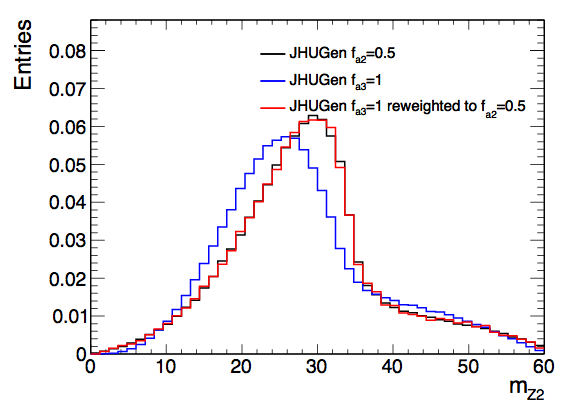
\includegraphics[width=0.4\textwidth]{reweightingvalidation/fa2halffa31} %\hfill
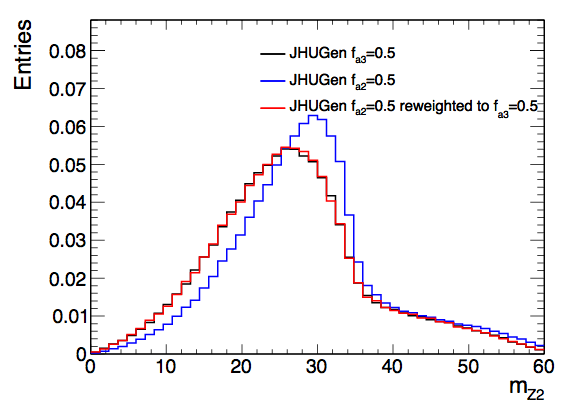
\includegraphics[width=0.4\textwidth]{reweightingvalidation/fa2halffa3half}\\
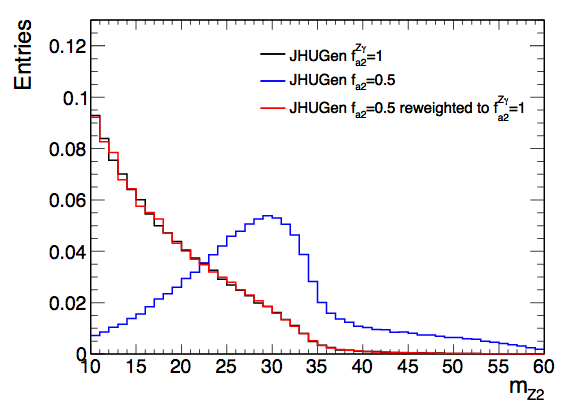
\includegraphics[width=0.4\textwidth]{reweightingvalidation/fa2Zgamma} %\hfill
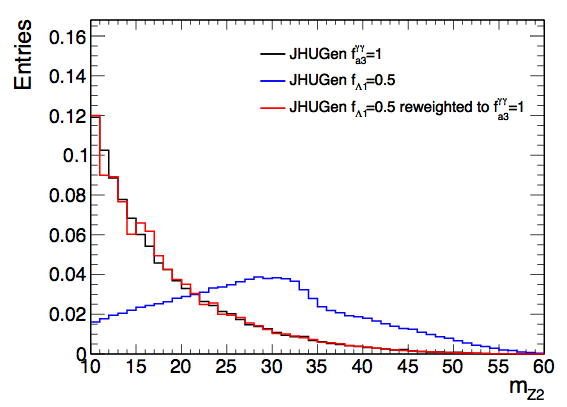
\includegraphics[width=0.4\textwidth]{reweightingvalidation/flambda1fa3Zgamma}
\end{frame}

\begin{frame}{Applications for discriminating CP properties}
\begin{columns}
\begin{column}{0.3\textwidth}

[Bolognesi, Gao, Gritsan, Melnikov, Schulze, Tran, Whitbeck] arXiv:1208.4018 \\

[Anderson, Bolognesi, Caola, Gao, Gritsan, Martin, Melnikov, Schulze, Tran, Whitbeck, Zhou] arXiv:1309.4819

\end{column}
\begin{column}{0.2\textwidth}
\foreach \plot in {HZZ4l,ZZHBB,HZZVBF}{
\includegraphics[width=\columnwidth]{snowmass/angles-\plot}
}
\end{column}
\begin{column}{0.5\textwidth}
\centering JHUGen vs. AnalyticMELA \\
%\tiny \phantom{-} \\ %hack so it doesn't indent
\foreach \plot in {phi,costhetastar,phistar1,costheta1}{
\foreach \spn in {spin0_3in1,spin1_2in1,spin2_3in1}{
\noindent\includegraphics[width=0.3\columnwidth]{onthespinandparity/\plot_125GeV_\spn}
}
\\
}
\end{column}
\end{columns}
\end{frame}

\begin{frame}{JHUGen in action: Generation, reweighting, discriminants}{
%twiki: https://twiki.cern.ch/twiki/bin/view/CMSPublic/Hig14018PaperTwiki
CMS analysis $H \to ZZ^*/Z\gamma^*/\gamma^*\gamma^* \to 4l$\hfill [CMS-HIG-14-018] arXiv:1411.3441
}
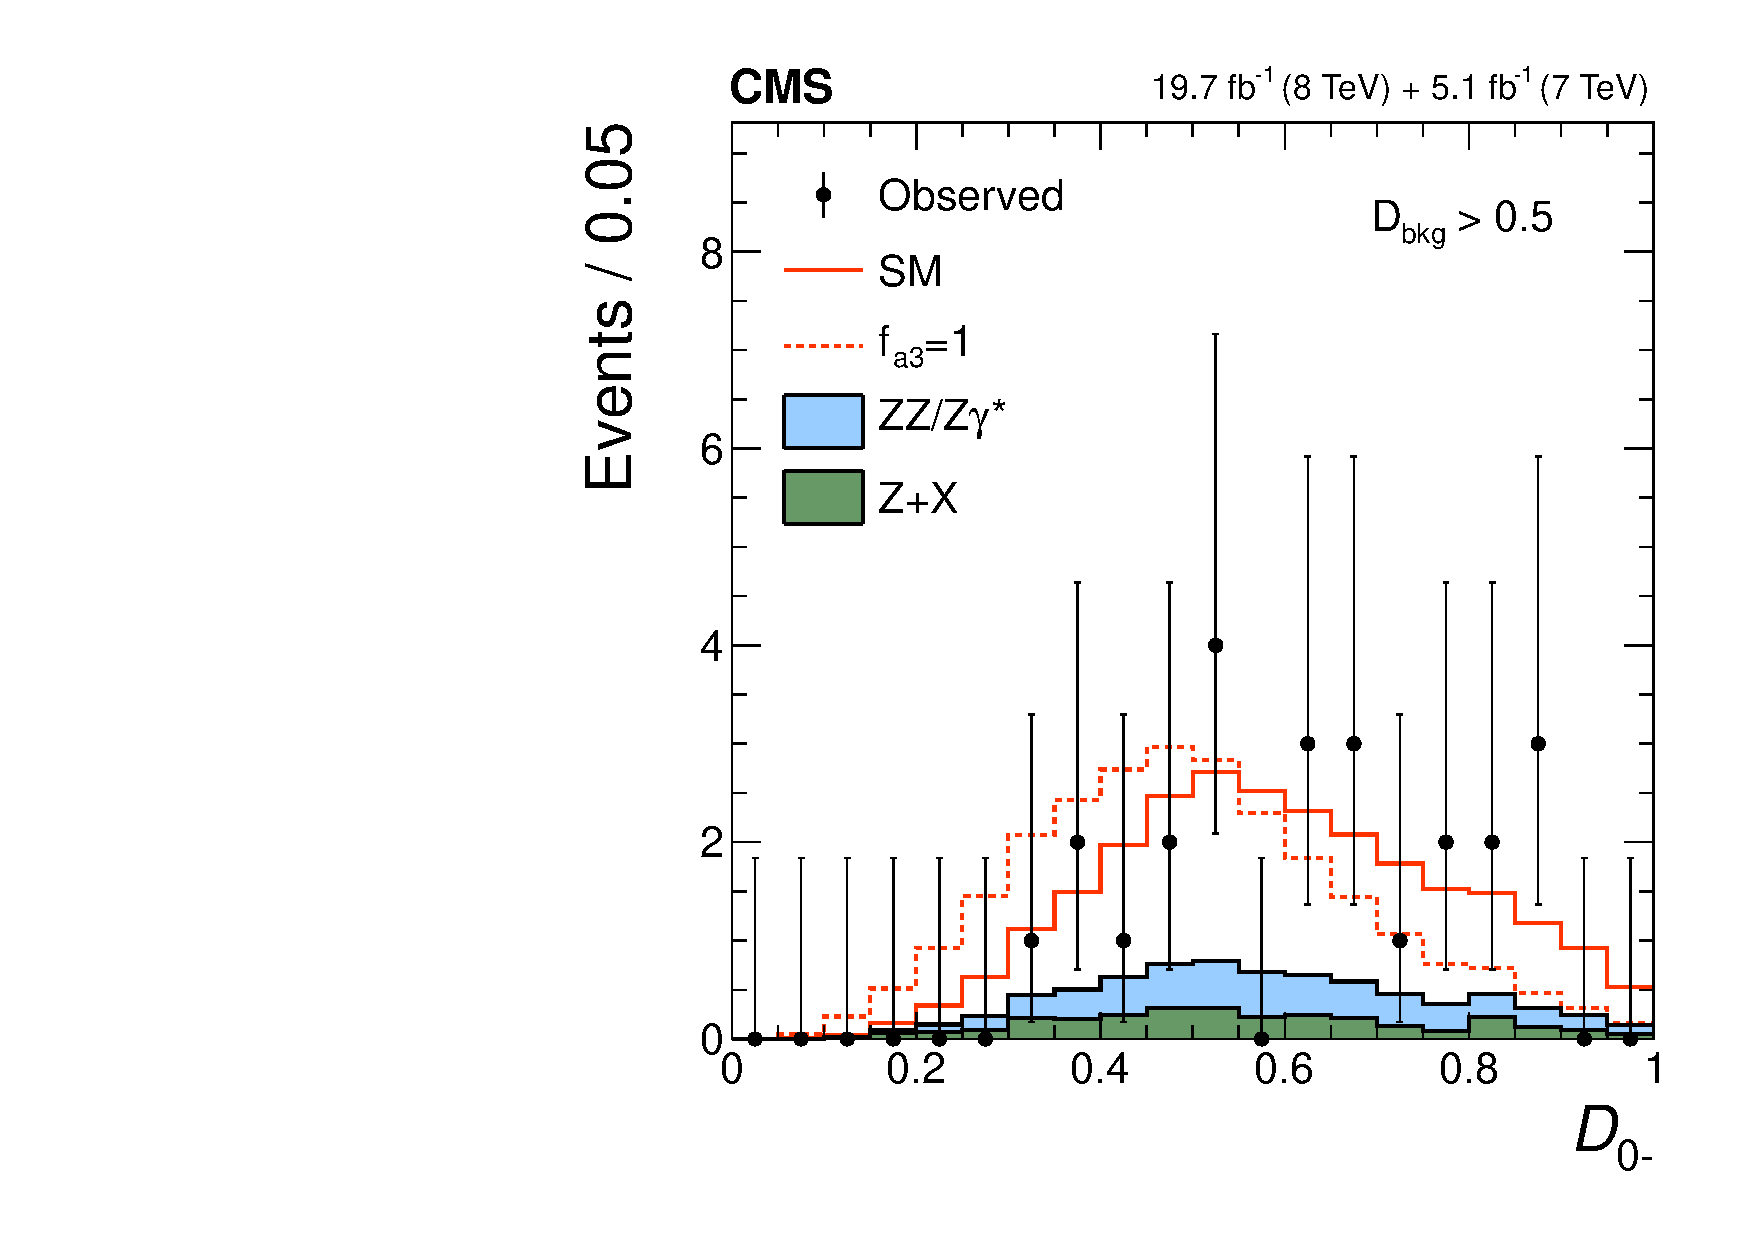
\includegraphics[width=0.25\textwidth]{HVV/d0minus}
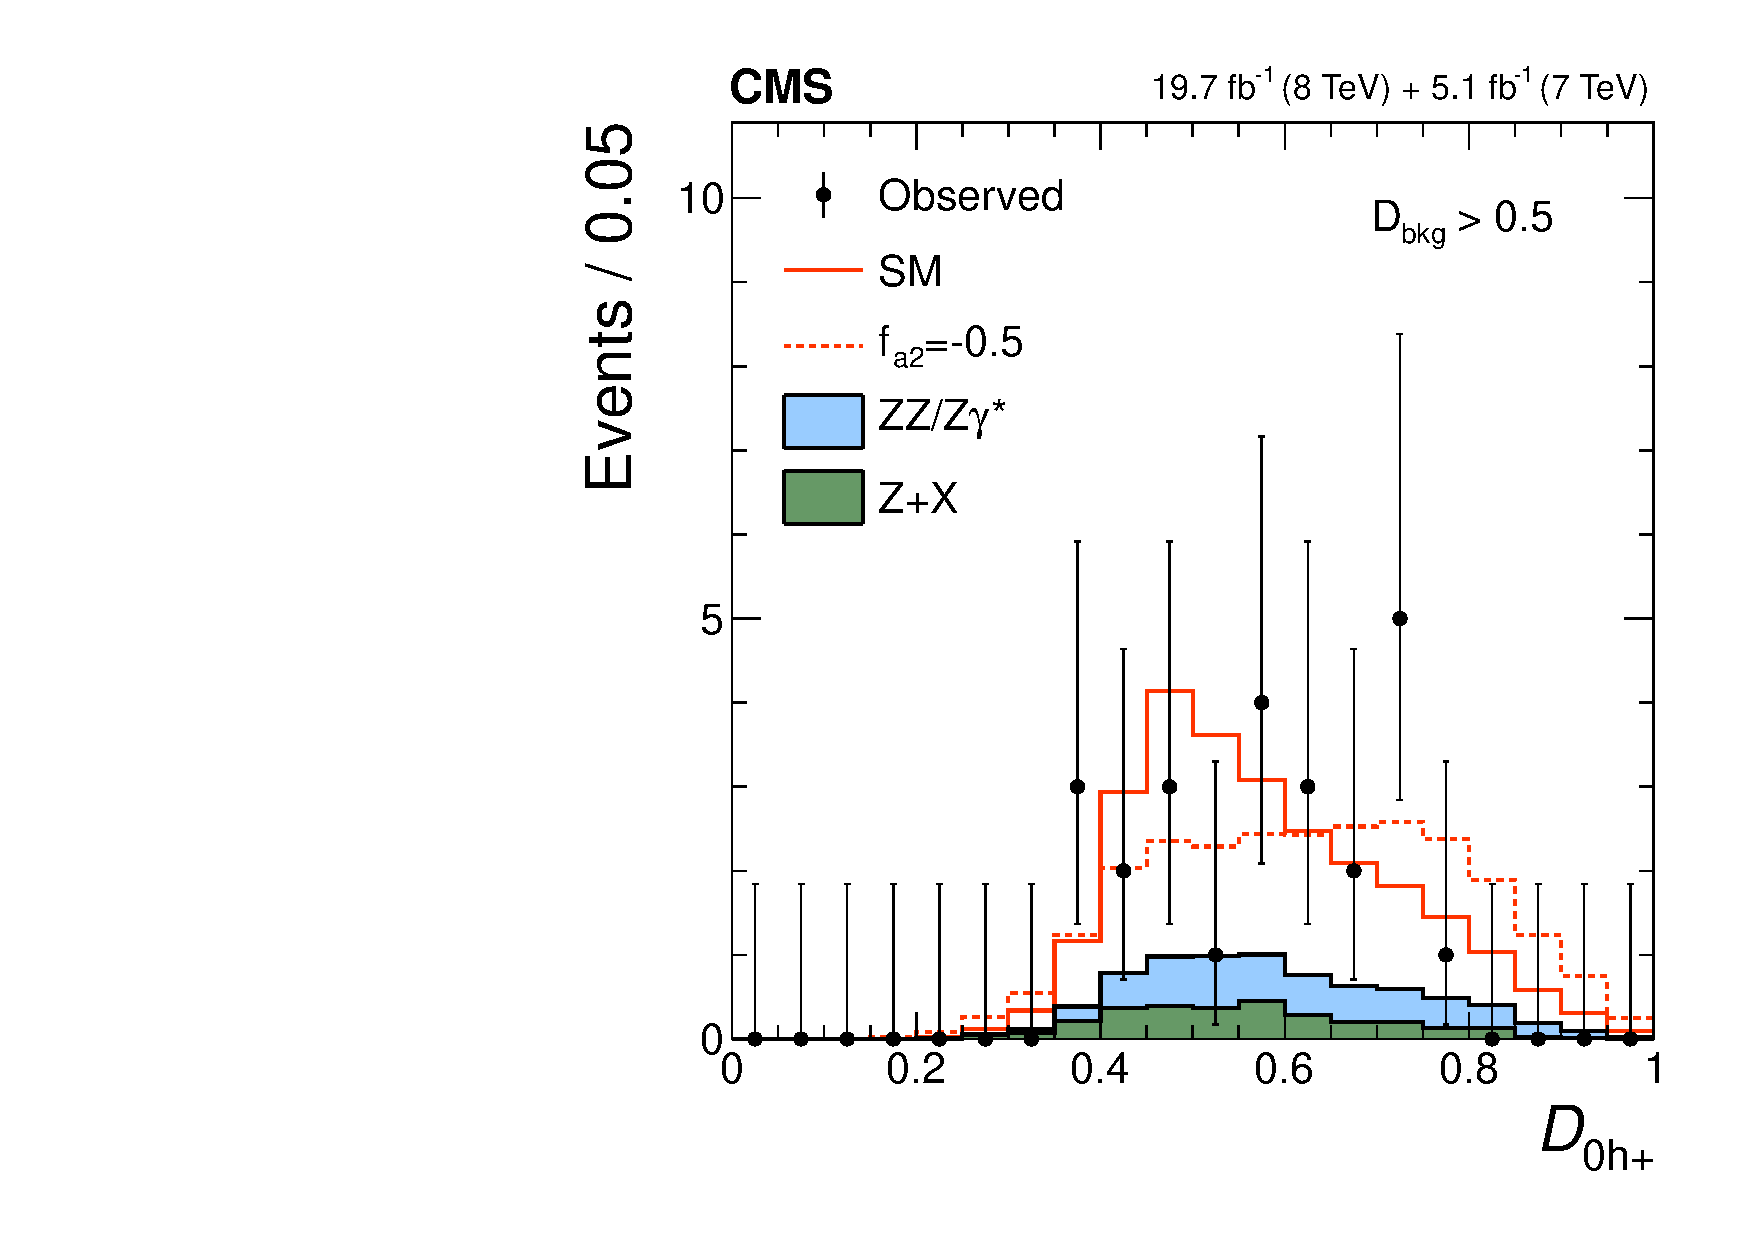
\includegraphics[width=0.25\textwidth]{HVV/d0hplus}
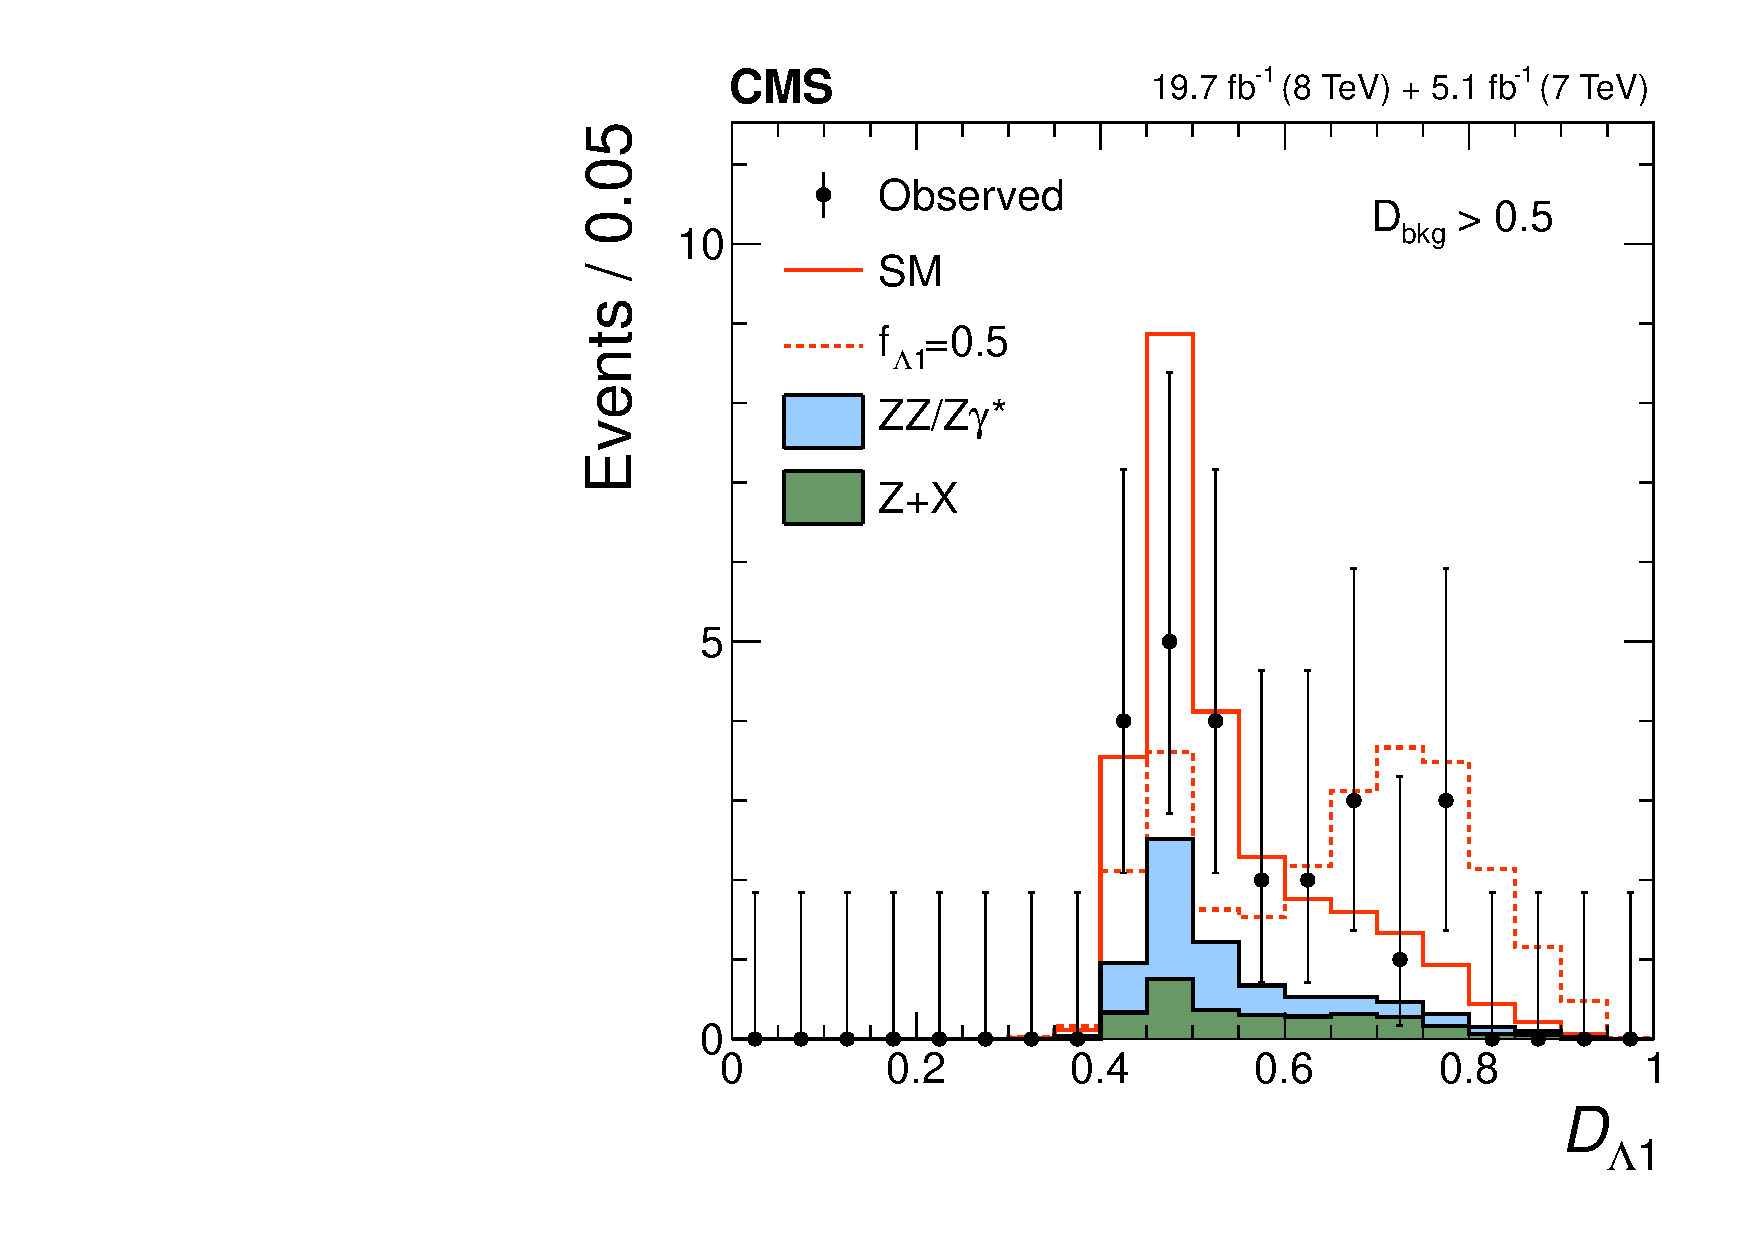
\includegraphics[width=0.25\textwidth]{HVV/dlambda1}
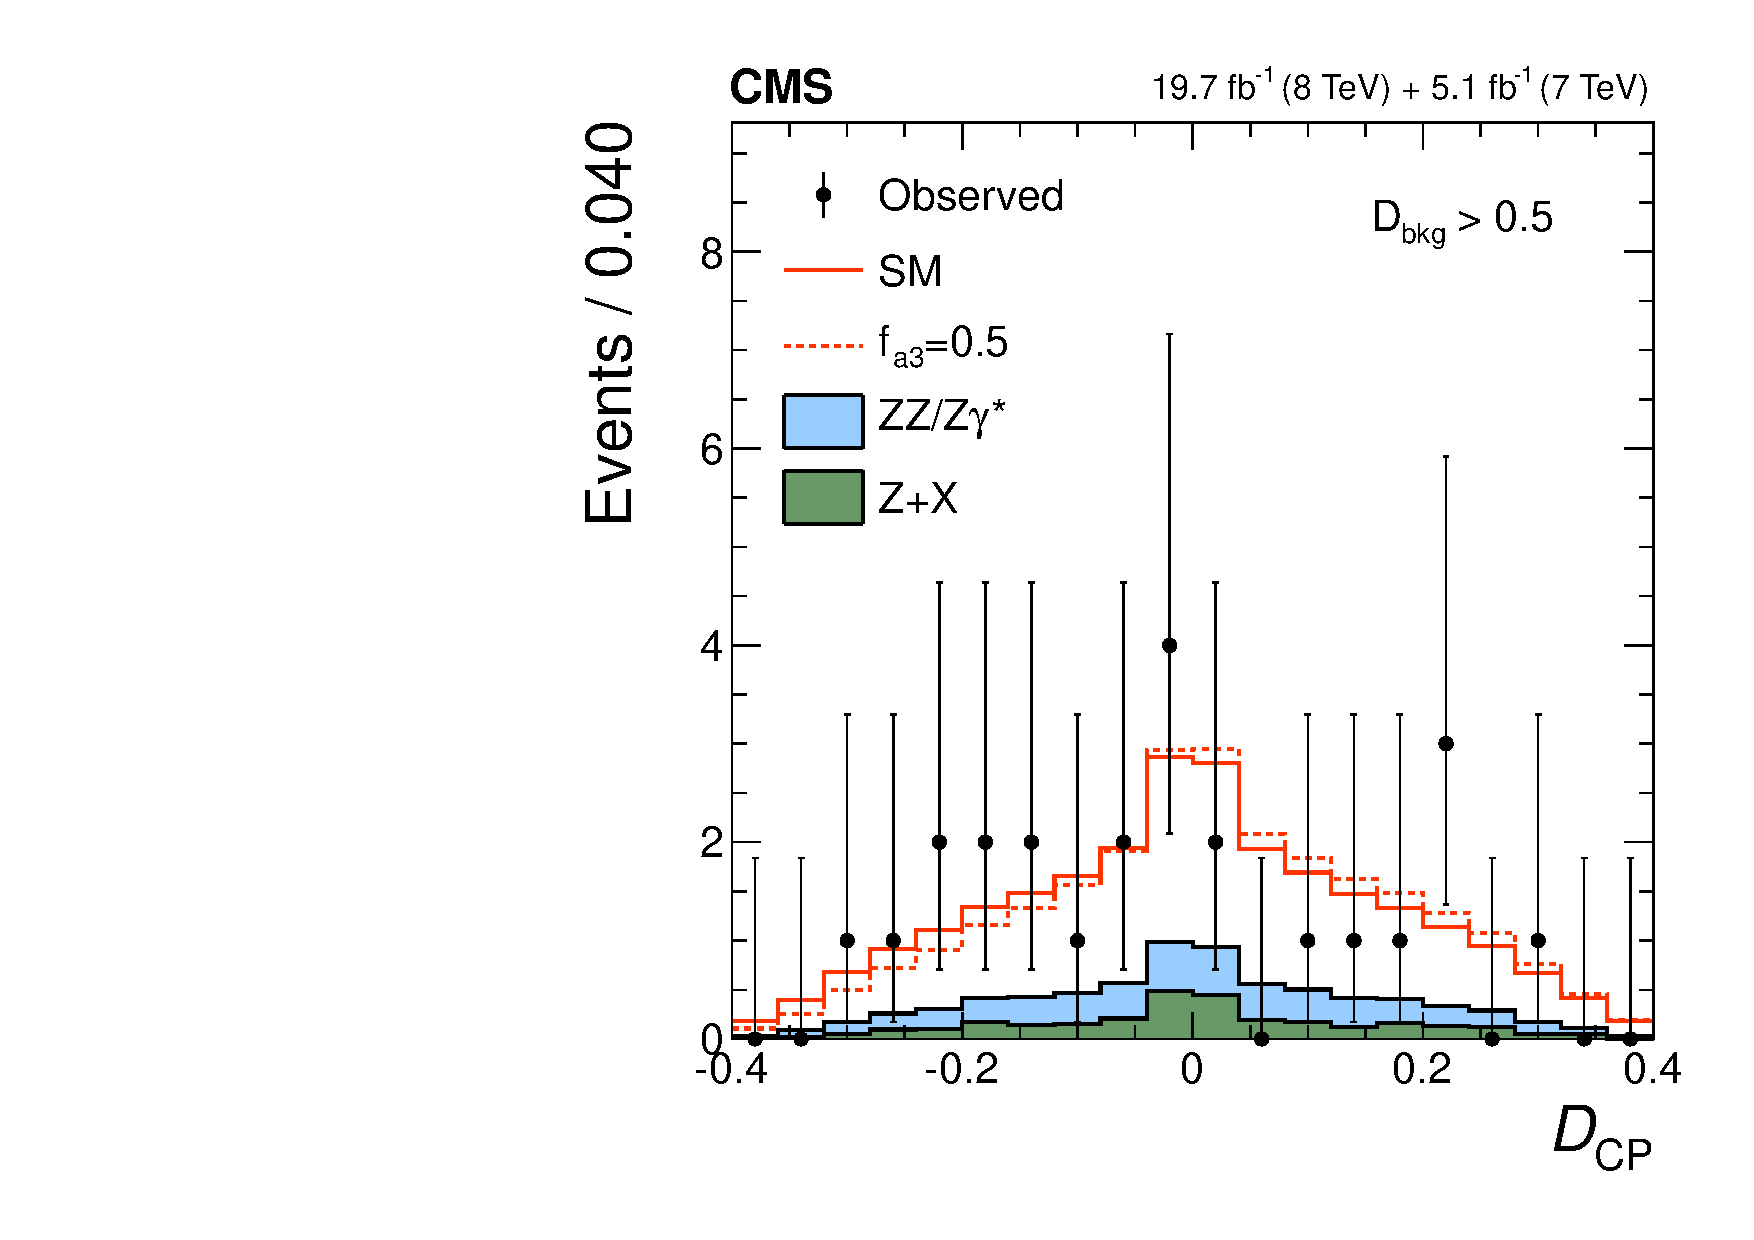
\includegraphics[width=0.25\textwidth]{HVV/dcp}
\\
\begin{columns}
\begin{column}{0.6\textwidth}
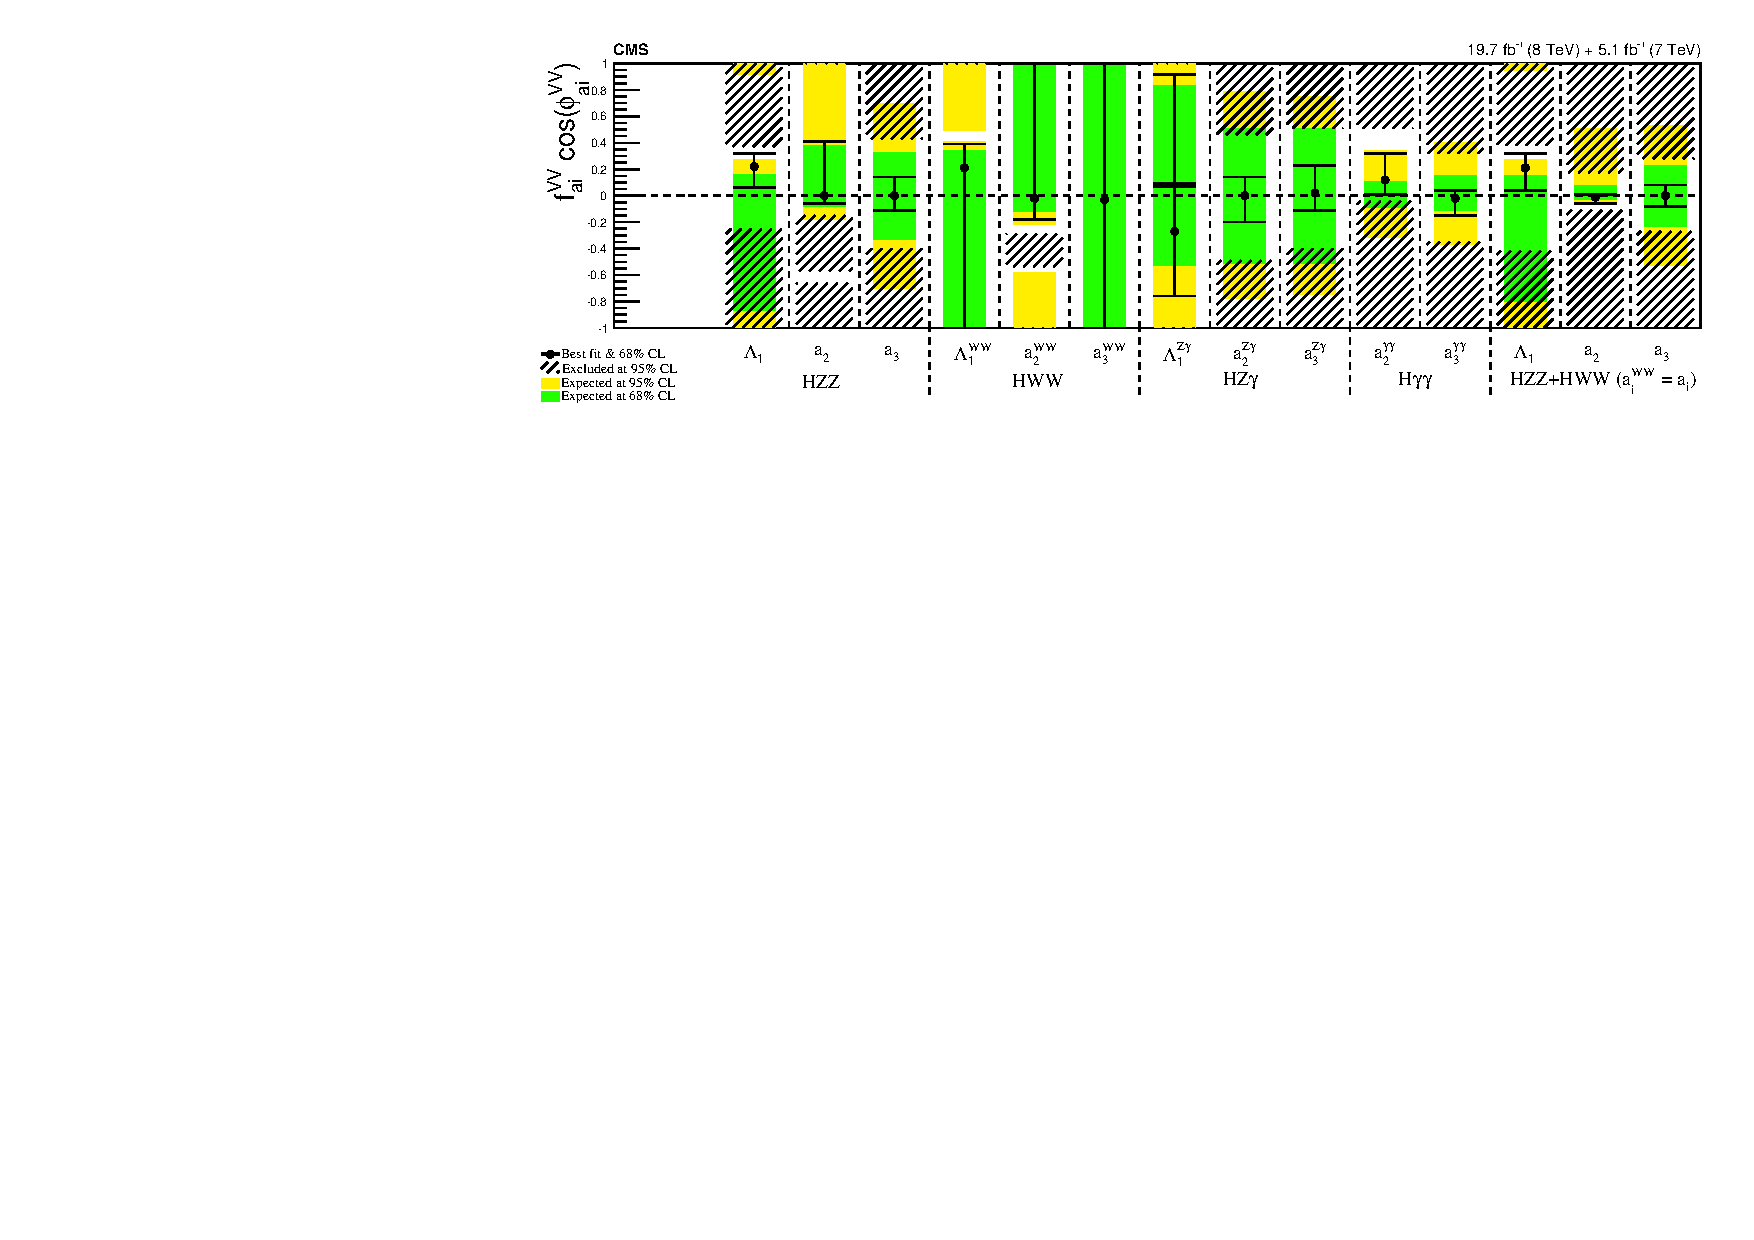
\includegraphics[width=\textwidth]{HVV/summary_a2a3lambda1}
\end{column}
\begin{column}{0.4\textwidth}
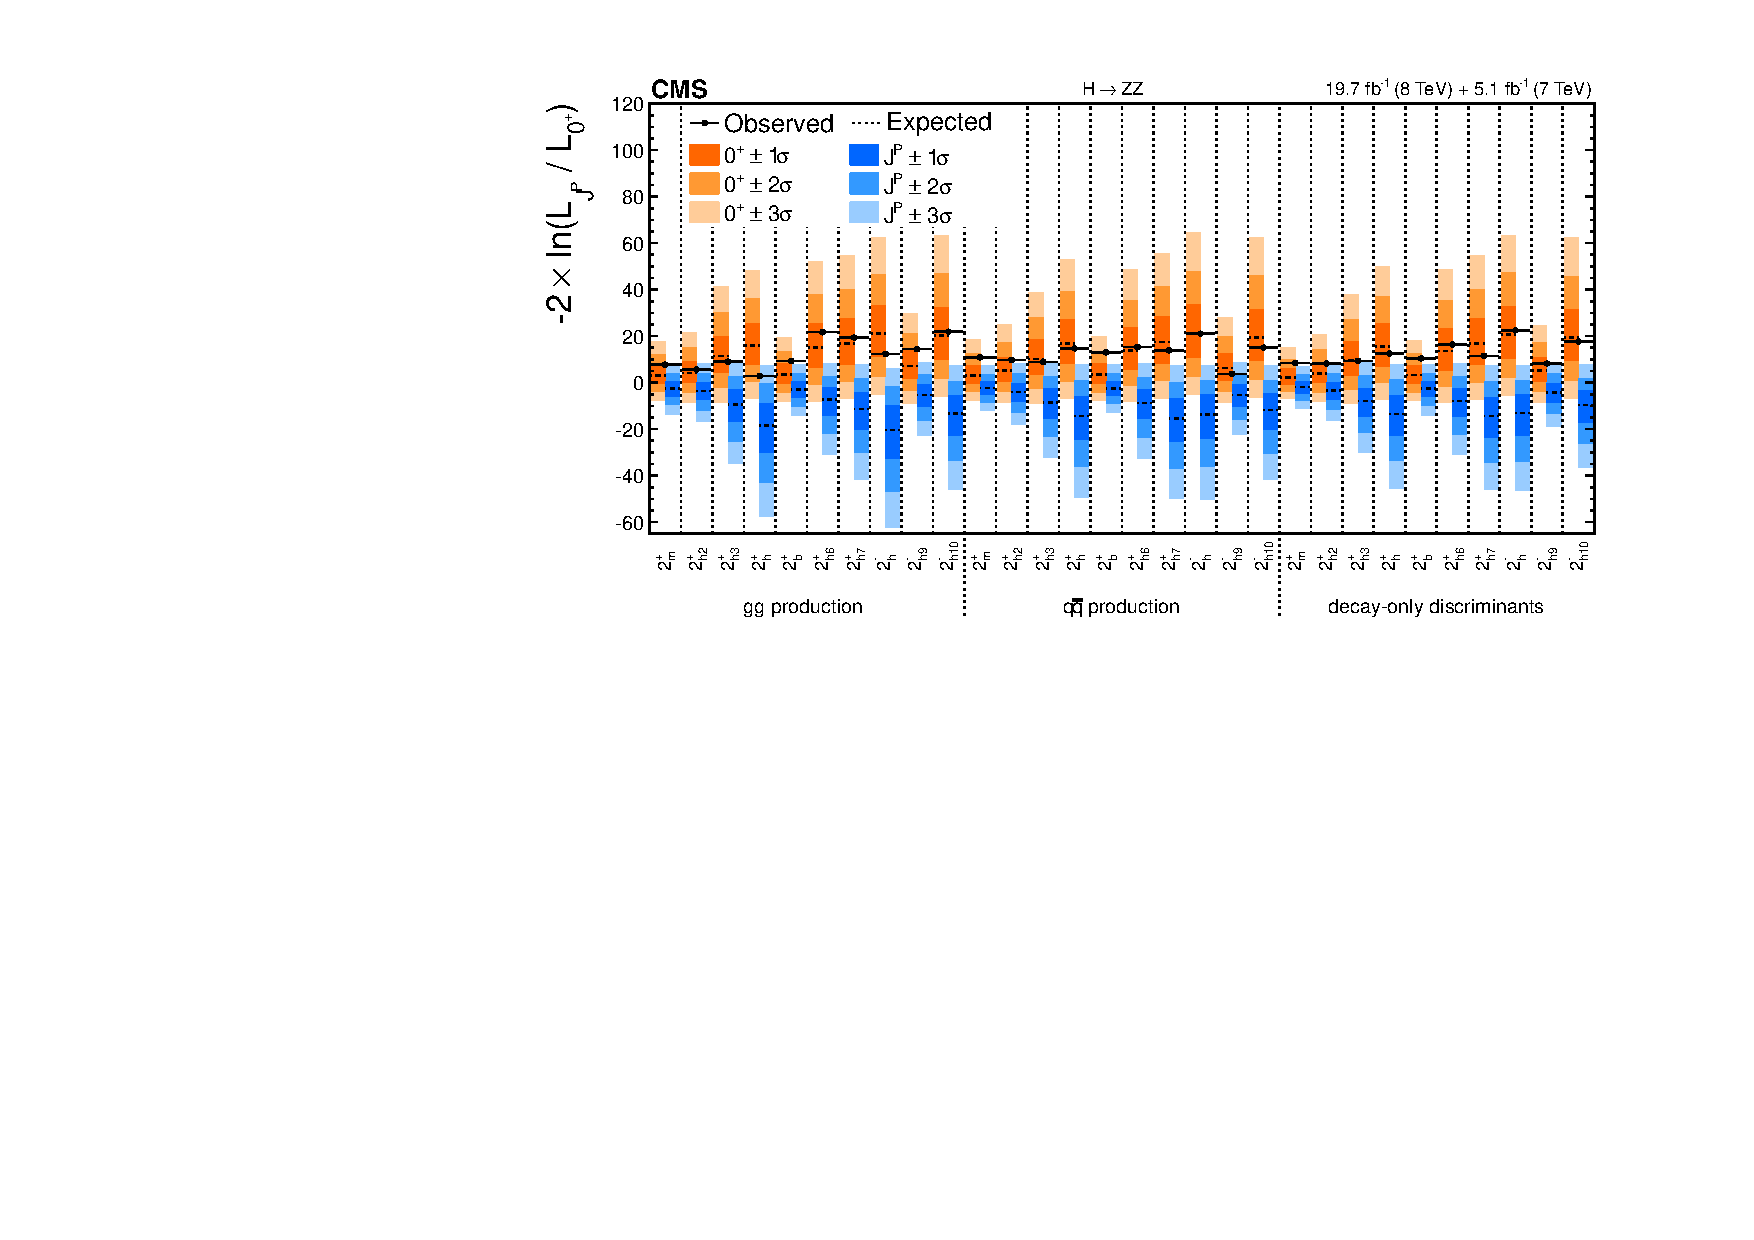
\includegraphics[width=\textwidth]{HVV/JP_SummaryPlot}
\end{column}
\end{columns}
\end{frame}

\begin{frame}{JHUGen in action: Applications of reweighting}{CMS analysis $H \to ZZ^*/Z\gamma^*/\gamma^*\gamma^* \to 4l$\hfill [CMS-HIG-14-018] arXiv:1411.3441}

JHUGen generator level:
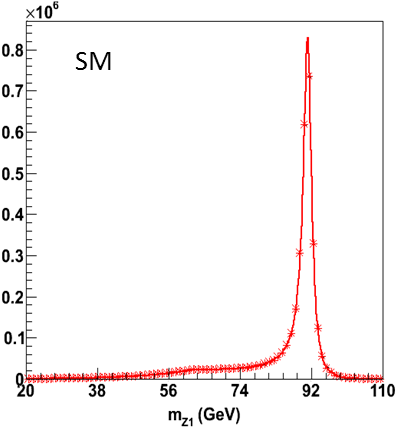
\includegraphics[width=0.25\textwidth]{HVV/SM}
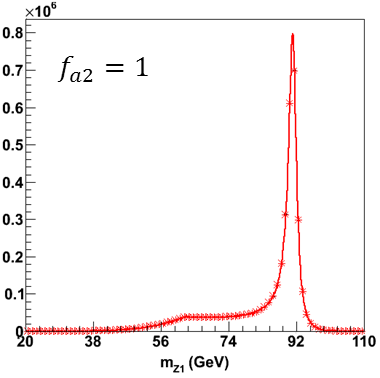
\includegraphics[width=0.25\textwidth]{HVV/fa2}
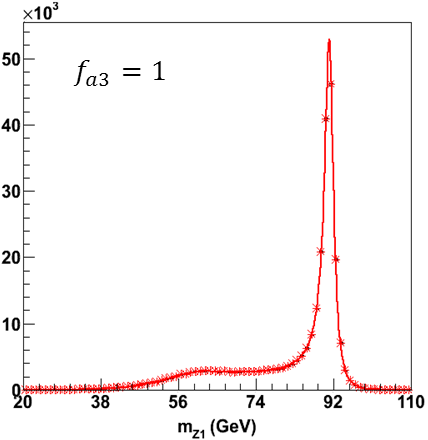
\includegraphics[width=0.25\textwidth]{HVV/fa3}
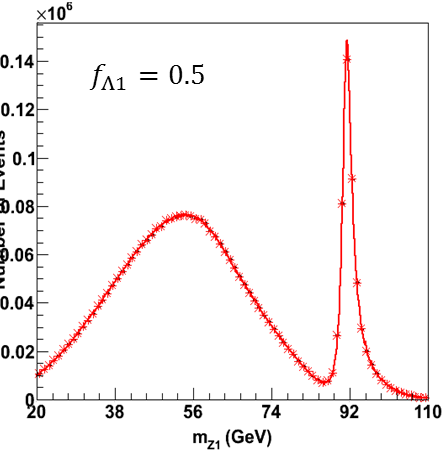
\includegraphics[width=0.25\textwidth]{HVV/flambda1}
\begin{columns}
\begin{column}{0.6\textwidth}
\footnotesize
\begin{itemize}
\item Generate 24 base models
\item Create 52 target models through reweighting
\item To increase statistics:
\begin{itemize}
\item Reweight \emph{everything to everything}
\end{itemize}
\item Effectively increase sample size by $\times 24$.
\end{itemize}
\end{column}
\begin{column}{0.13\textwidth} \footnotesize
JHUGen detector level (everything reweighted to SM):
\end{column}
\begin{column}{0.27\textwidth}
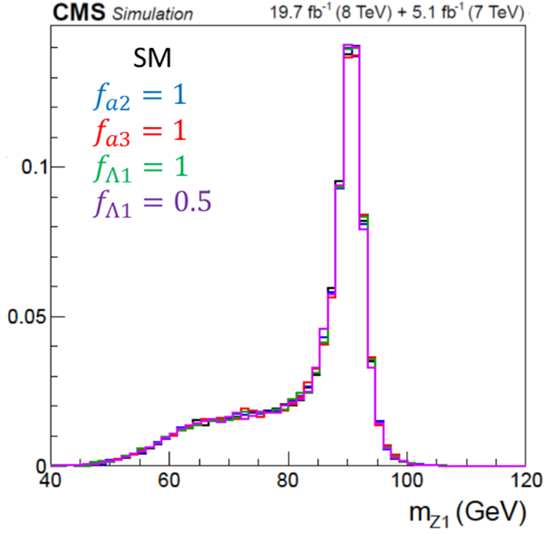
\includegraphics[width=\textwidth]{HVV/reweighted}
\end{column}
\end{columns}
\end{frame}

\begin{frame}{JHUGen in action}{CMS analysis $H \to ZZ^*/Z\gamma^*/\gamma^*\gamma^* \to 4l$\hfill [CMS-HIG-14-018] arXiv:1411.3441}
\begin{columns}
\begin{column}{0.6\textwidth}
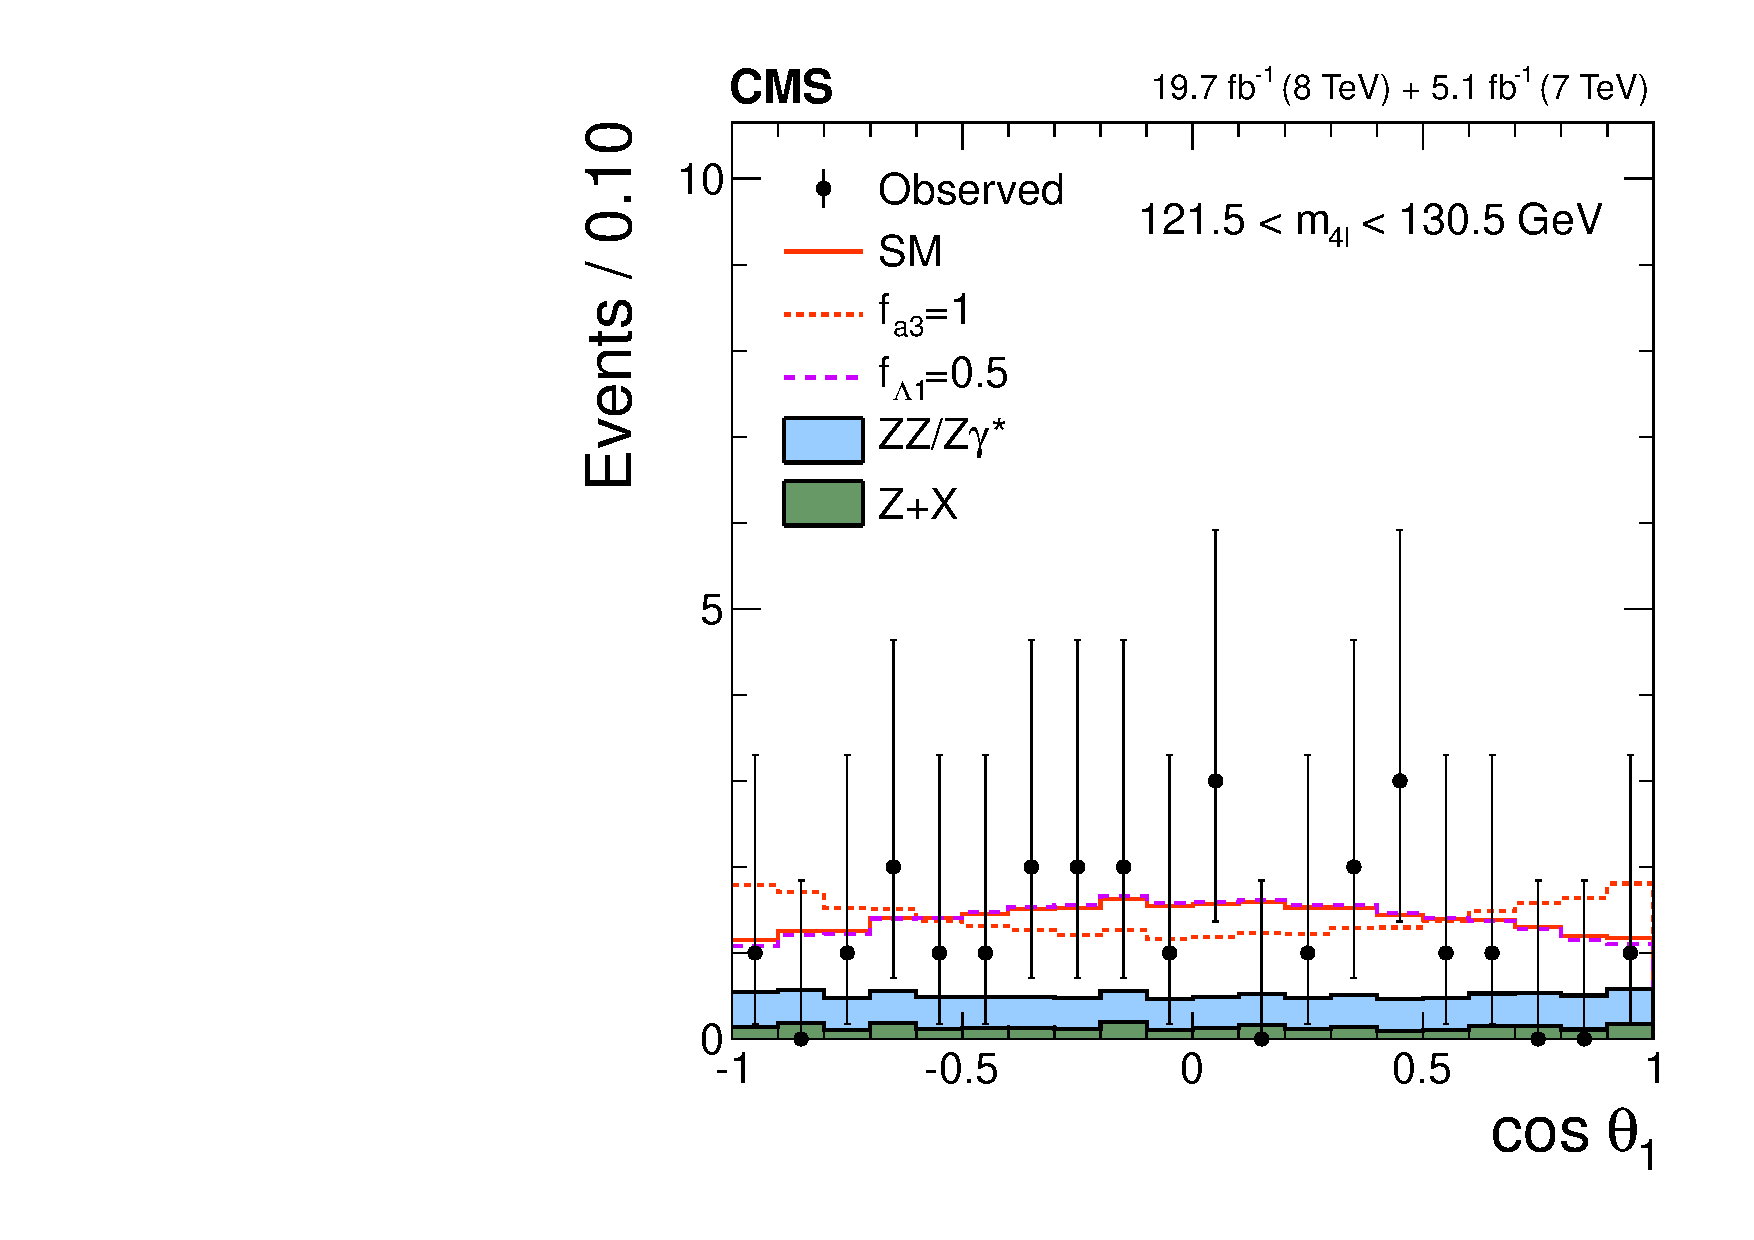
\includegraphics[width=.5\columnwidth]{HVV/costheta1}
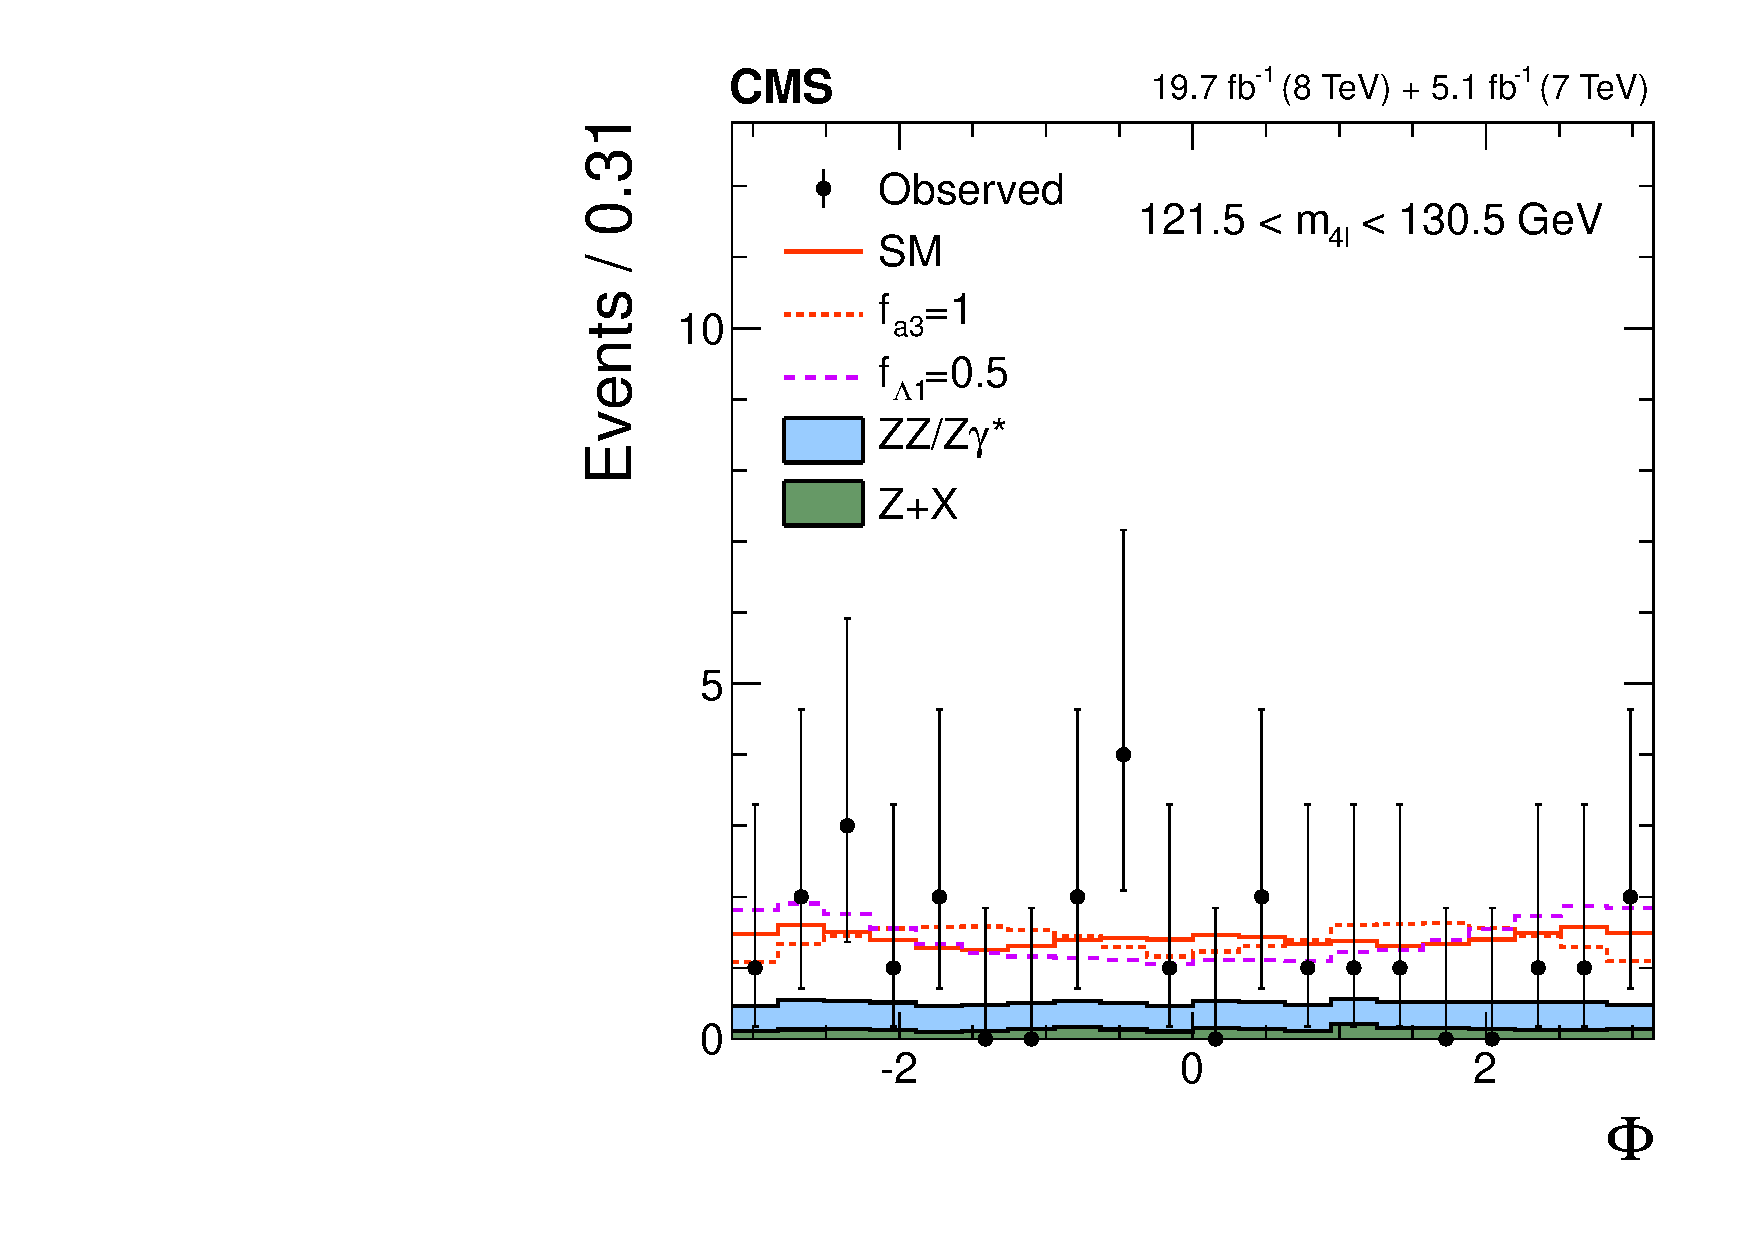
\includegraphics[width=.5\columnwidth]{HVV/Phi} \\
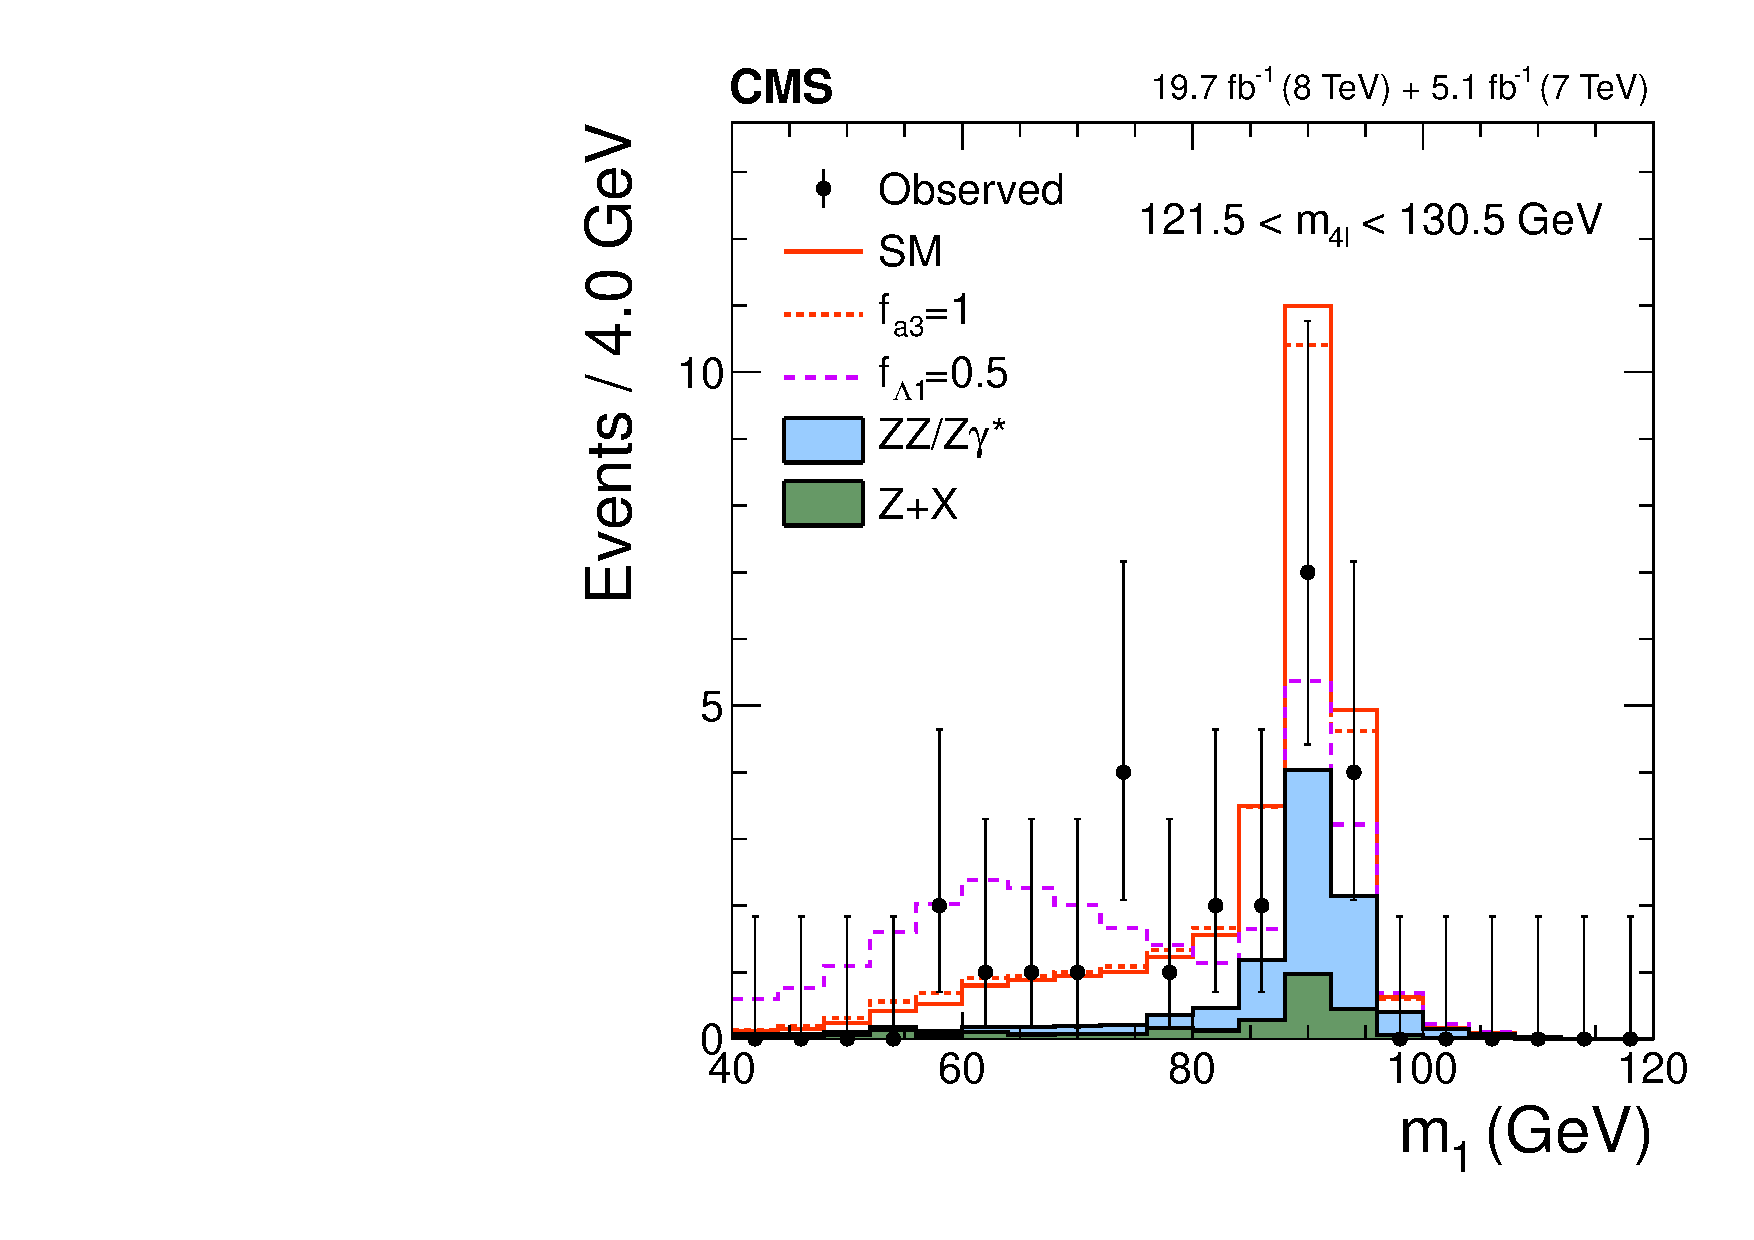
\includegraphics[width=.5\columnwidth]{HVV/m1}
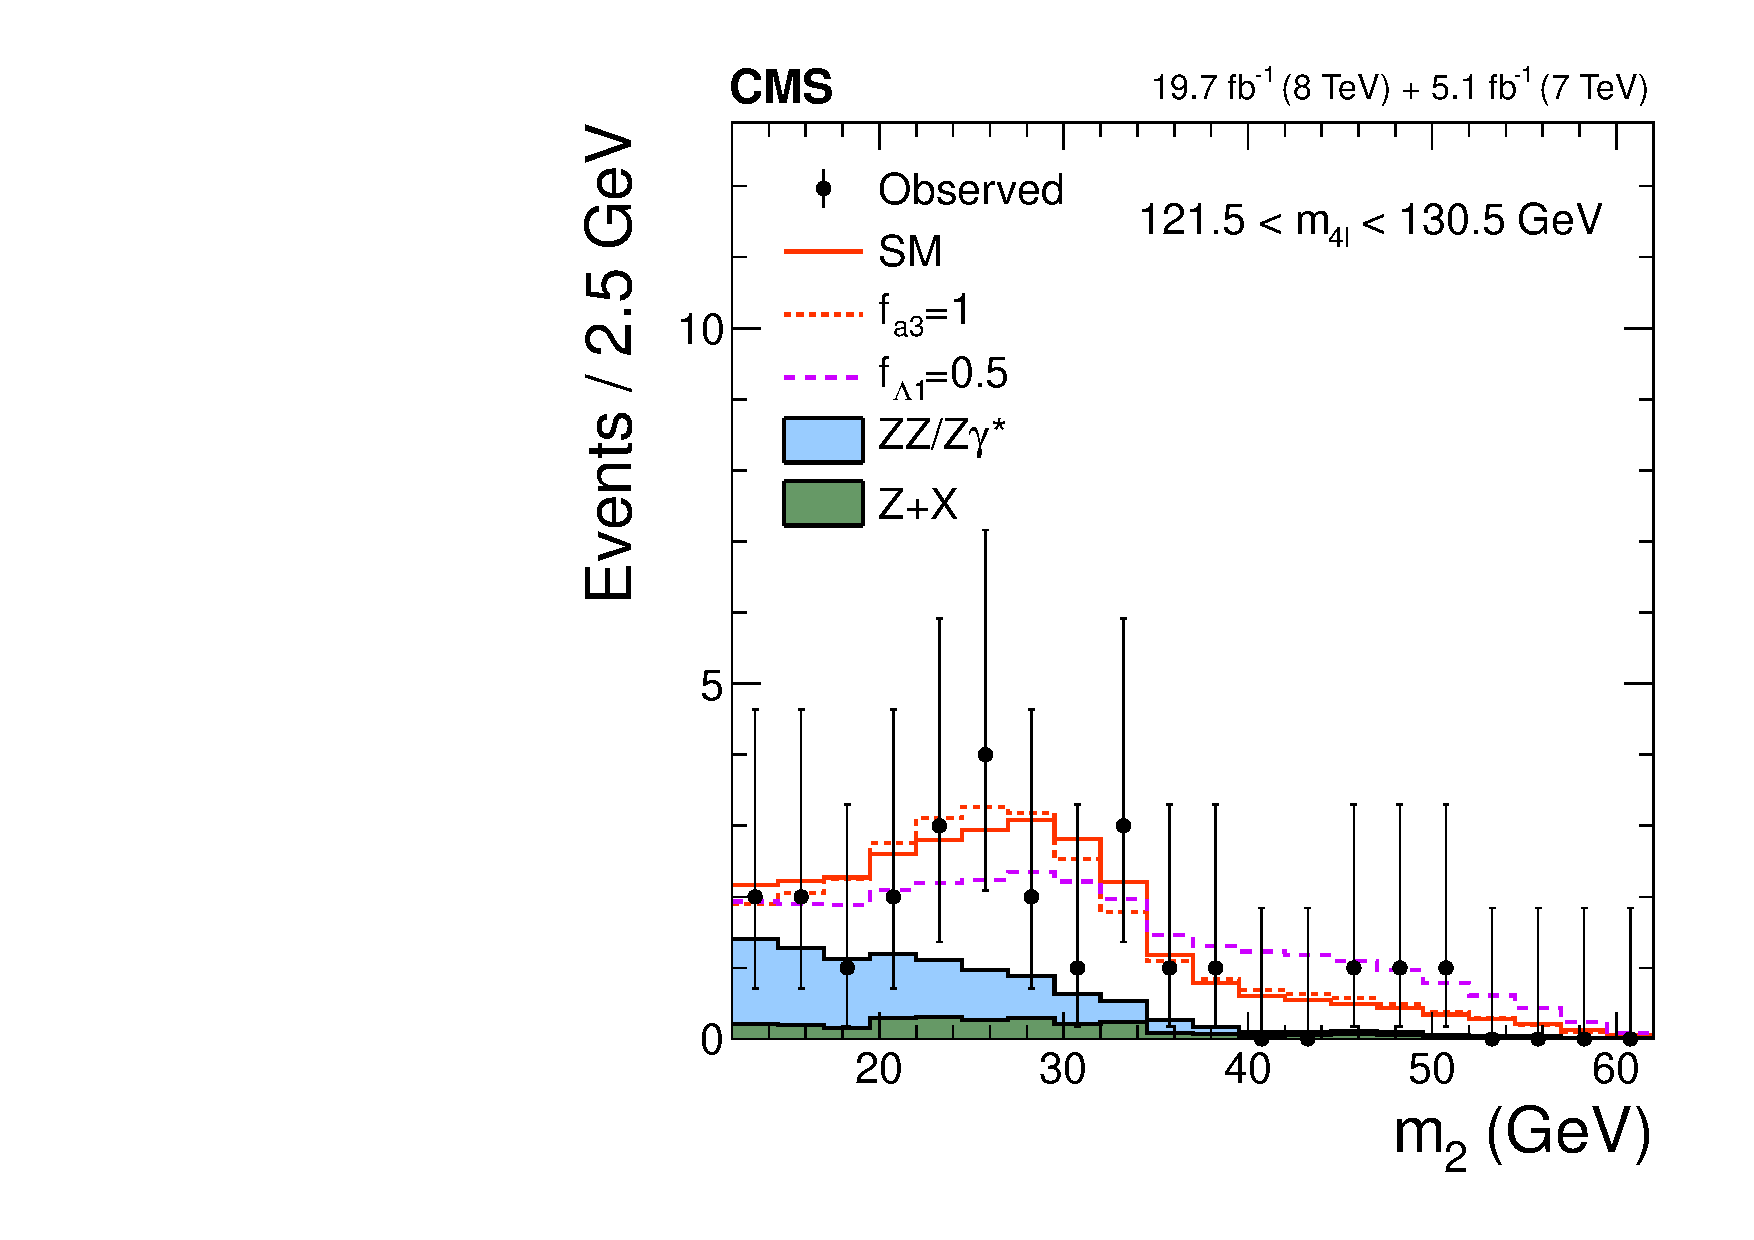
\includegraphics[width=.5\columnwidth]{HVV/m2}
\end{column}
\begin{column}{0.4\textwidth}
\begin{itemize}
\item angular and mass variables for on-shell kinematics
\item all signal distributions obtained via reweighting
\end{itemize}
\end{column}
\end{columns}
\end{frame}

\begin{frame}{JHUGen in action}{CMS analysis $H \to ZZ^*/Z\gamma^*/\gamma^*\gamma^* \to 4l$\hfill [CMS-HIG-14-018] arXiv:1411.3441}
\begin{columns}
\begin{column}{0.6\textwidth}
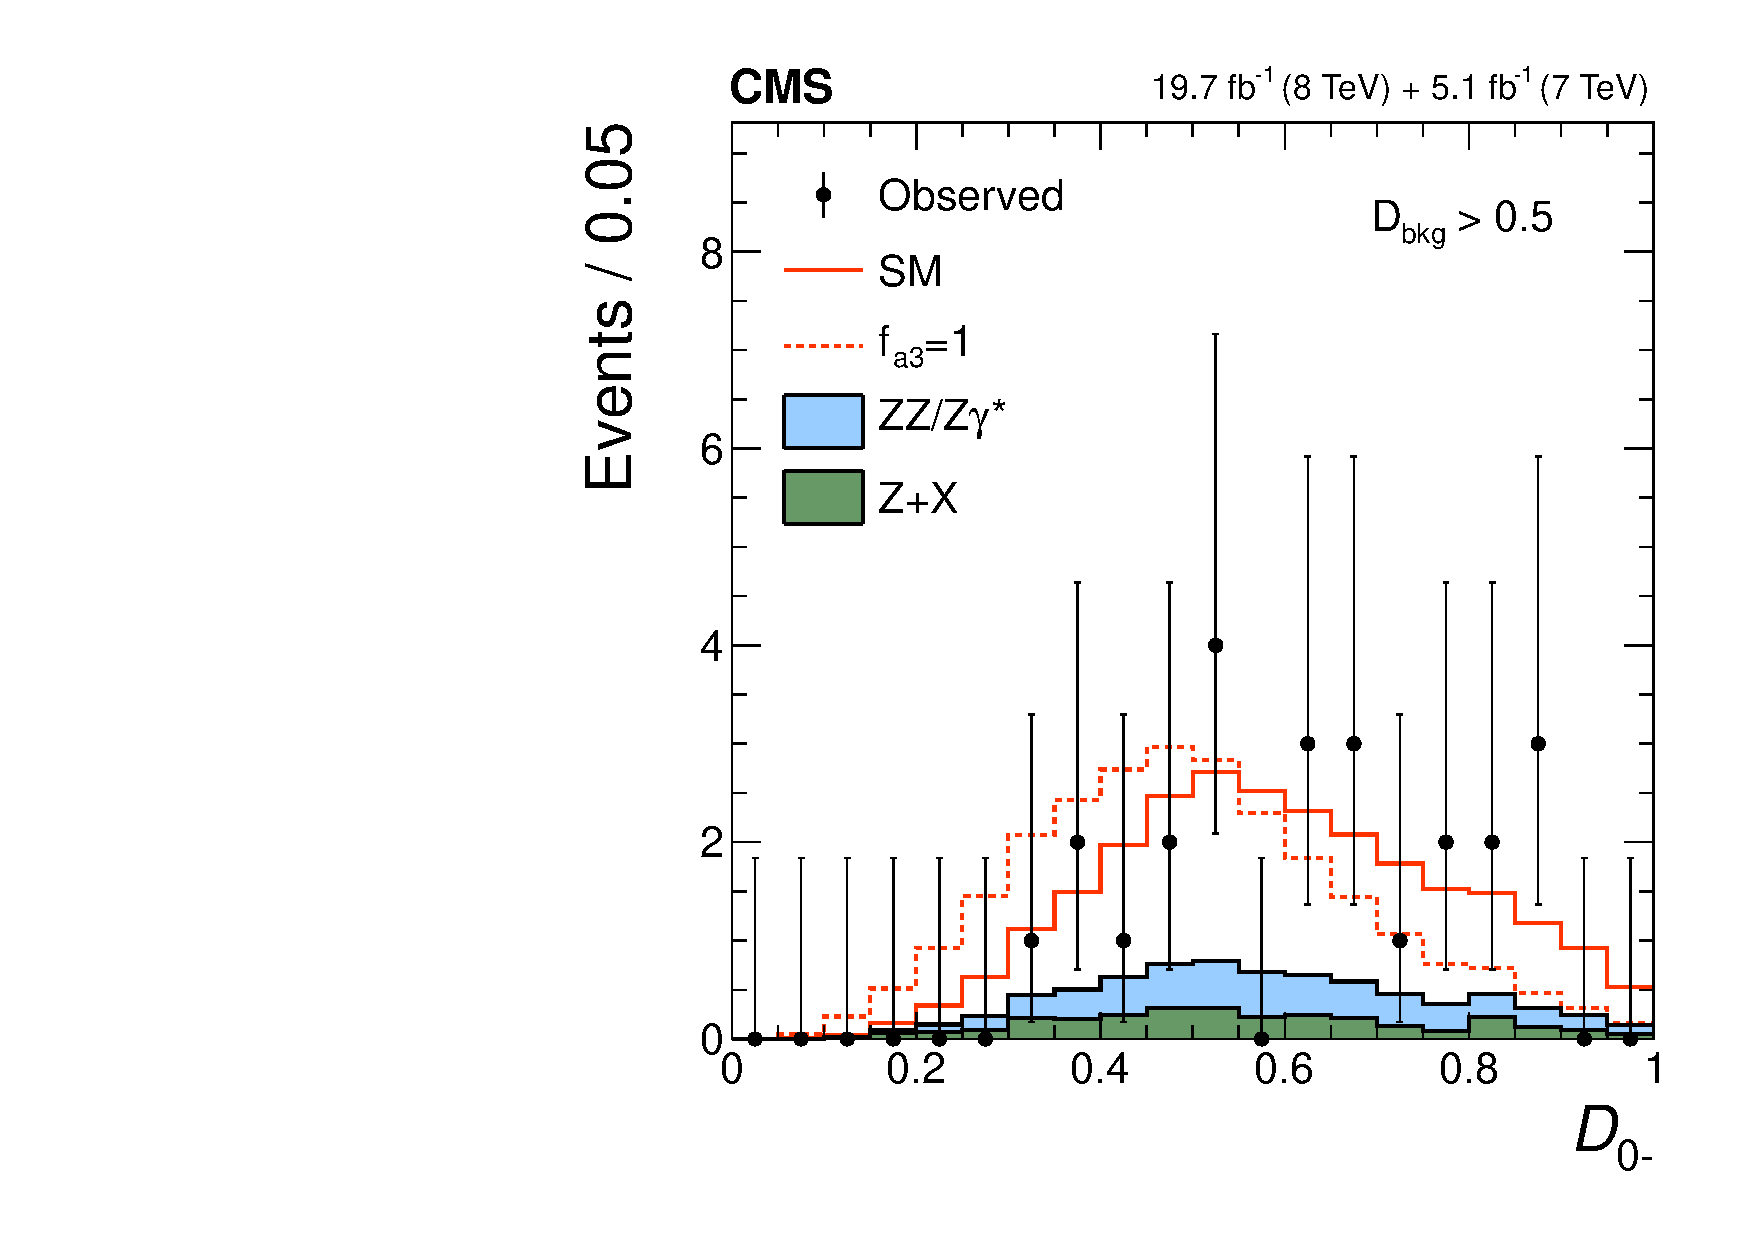
\includegraphics[width=.5\columnwidth]{HVV/d0minus}
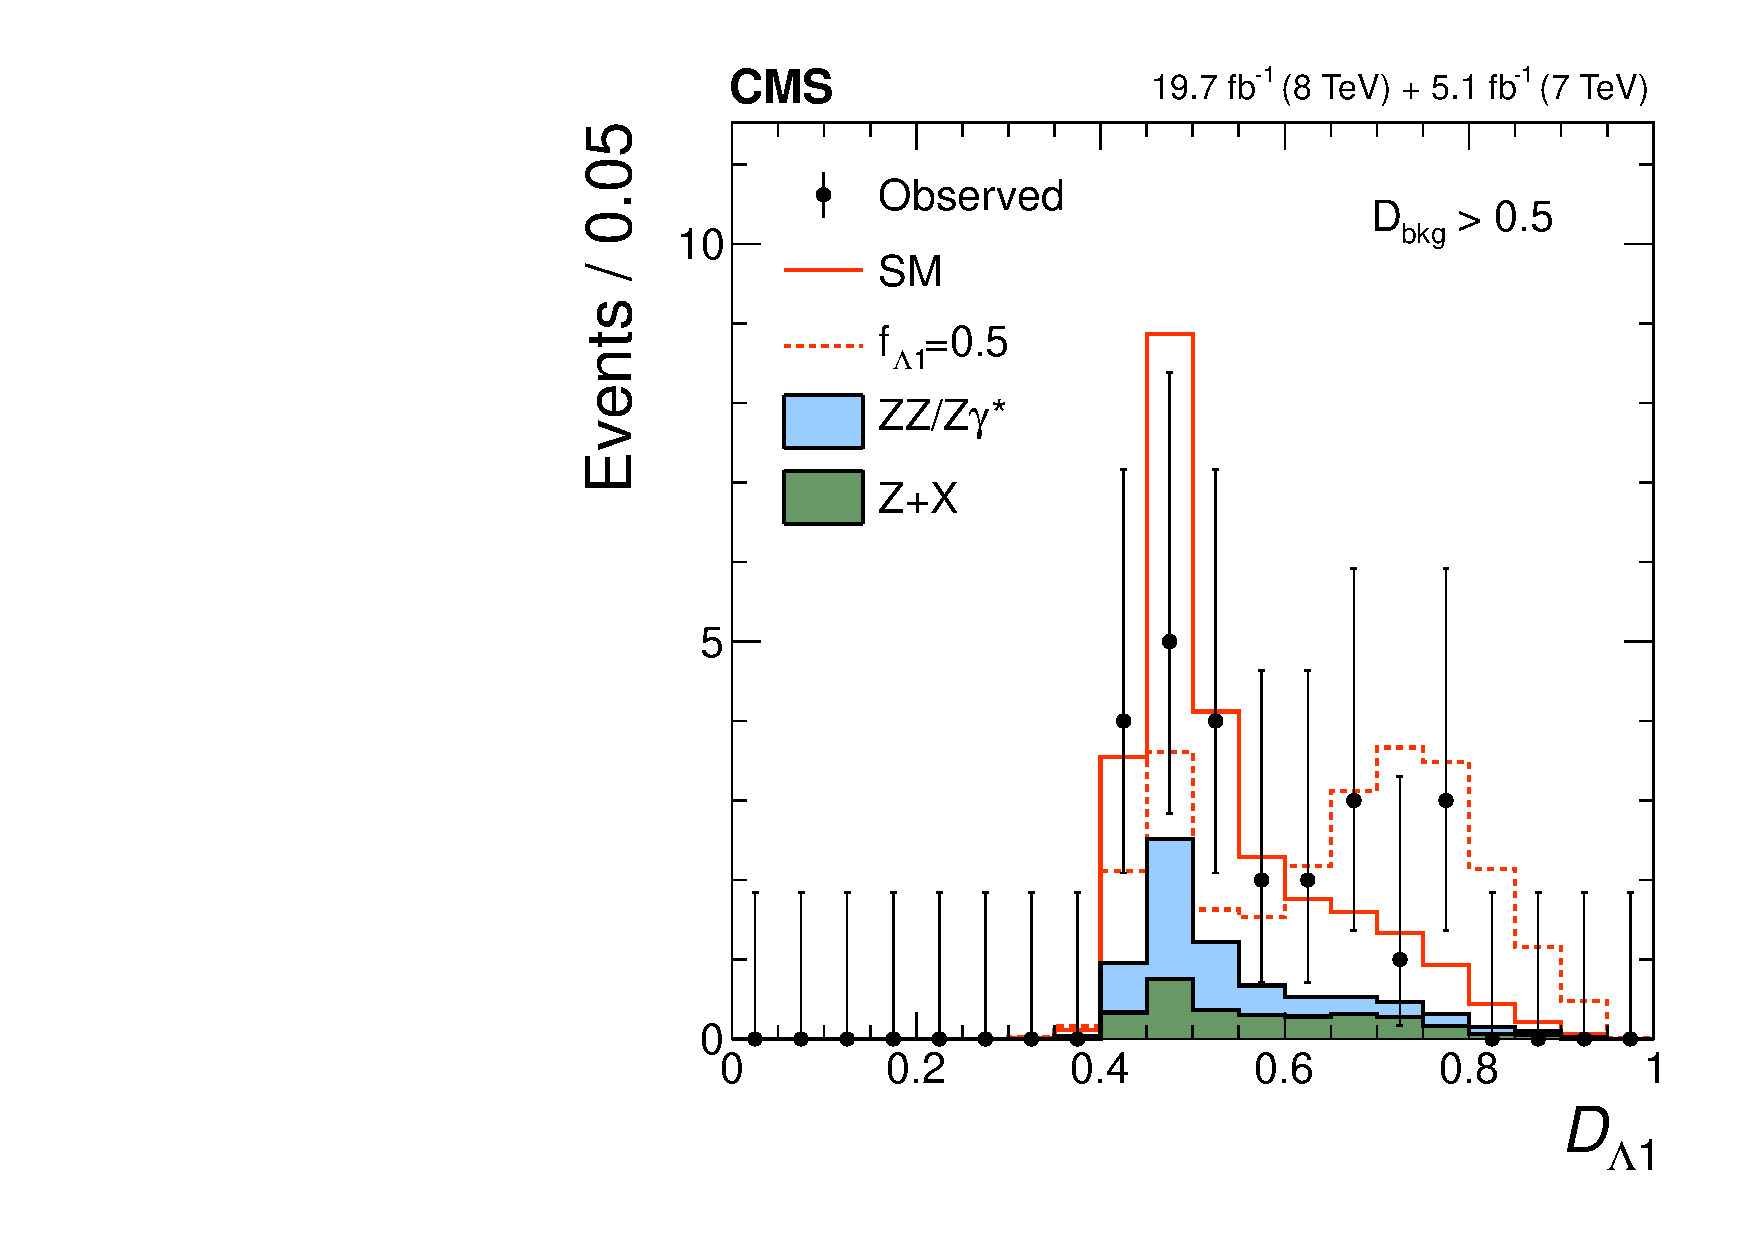
\includegraphics[width=.5\columnwidth]{HVV/dlambda1} \\
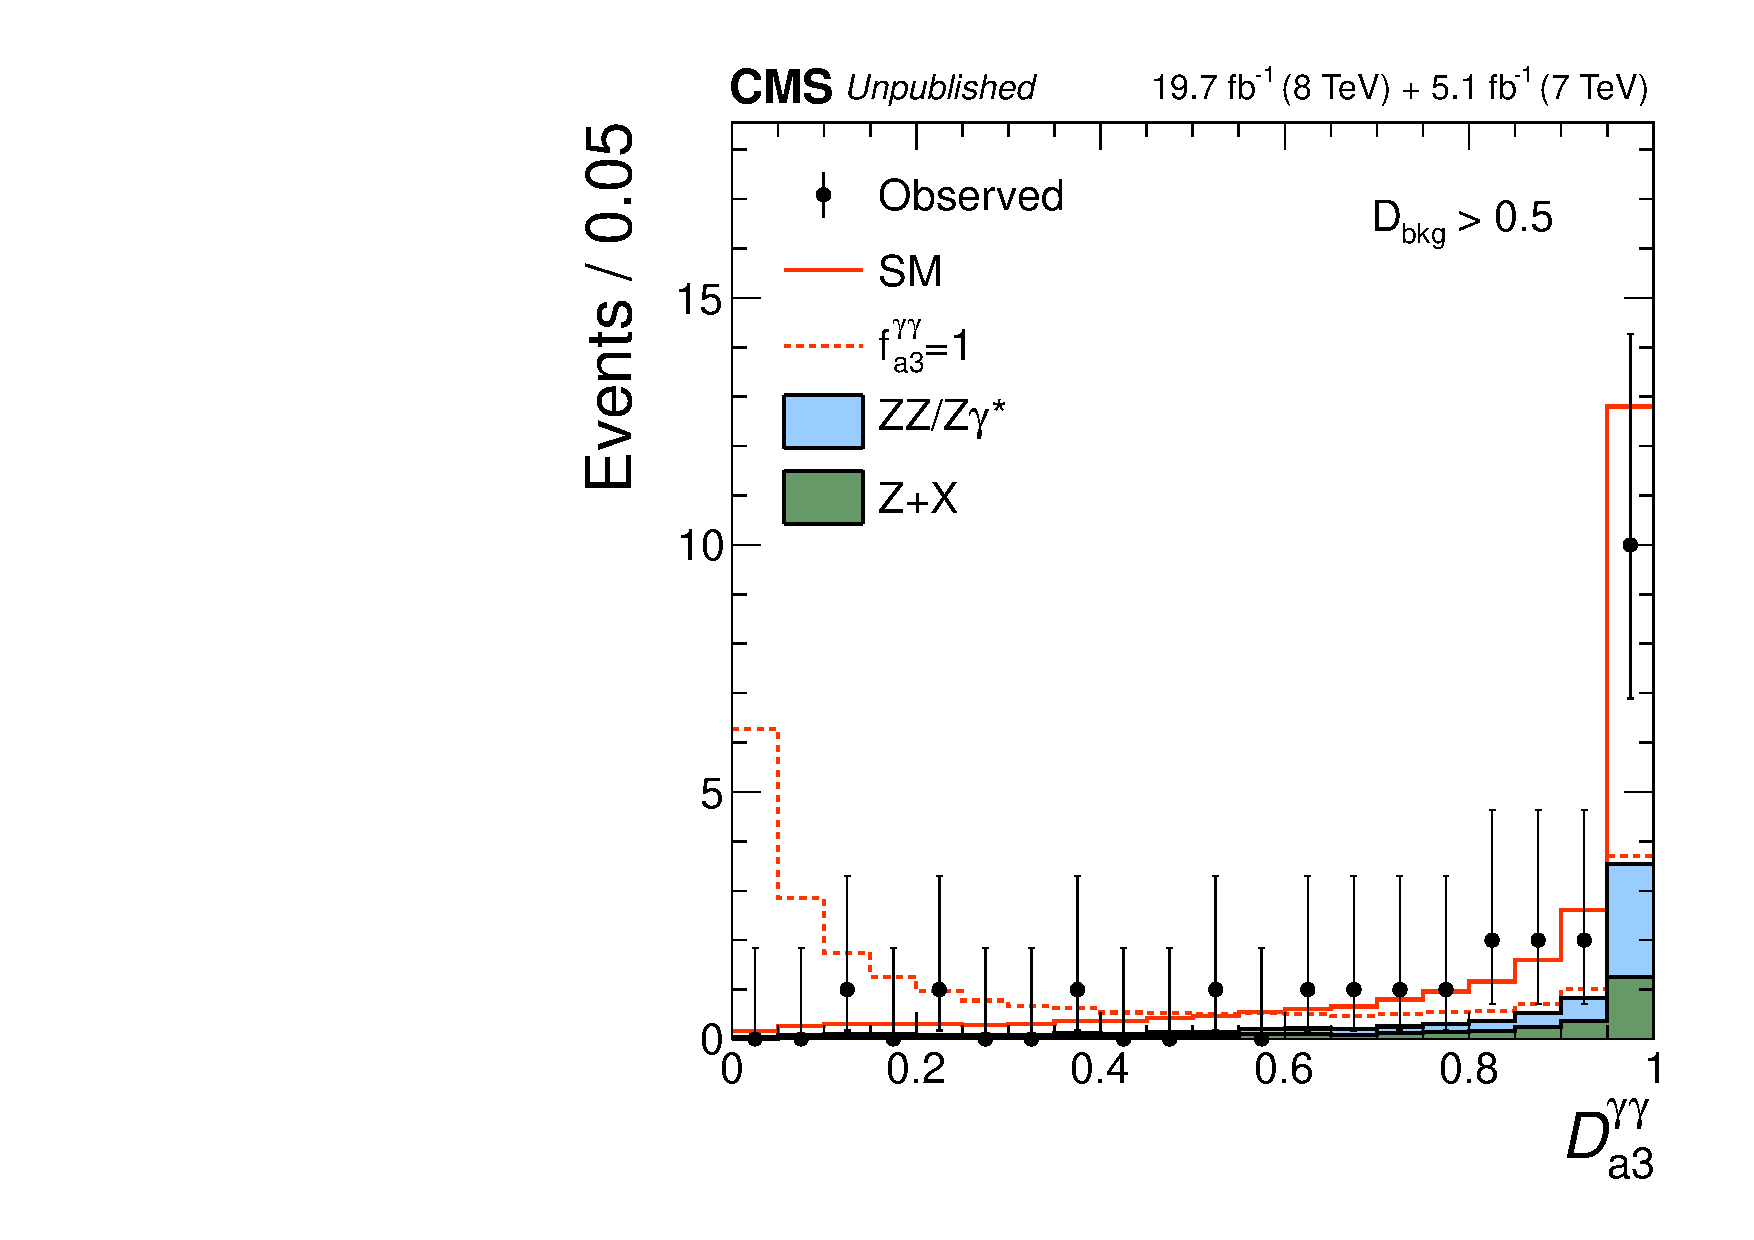
\includegraphics[width=.5\columnwidth]{HVV/Da3gammagamma}
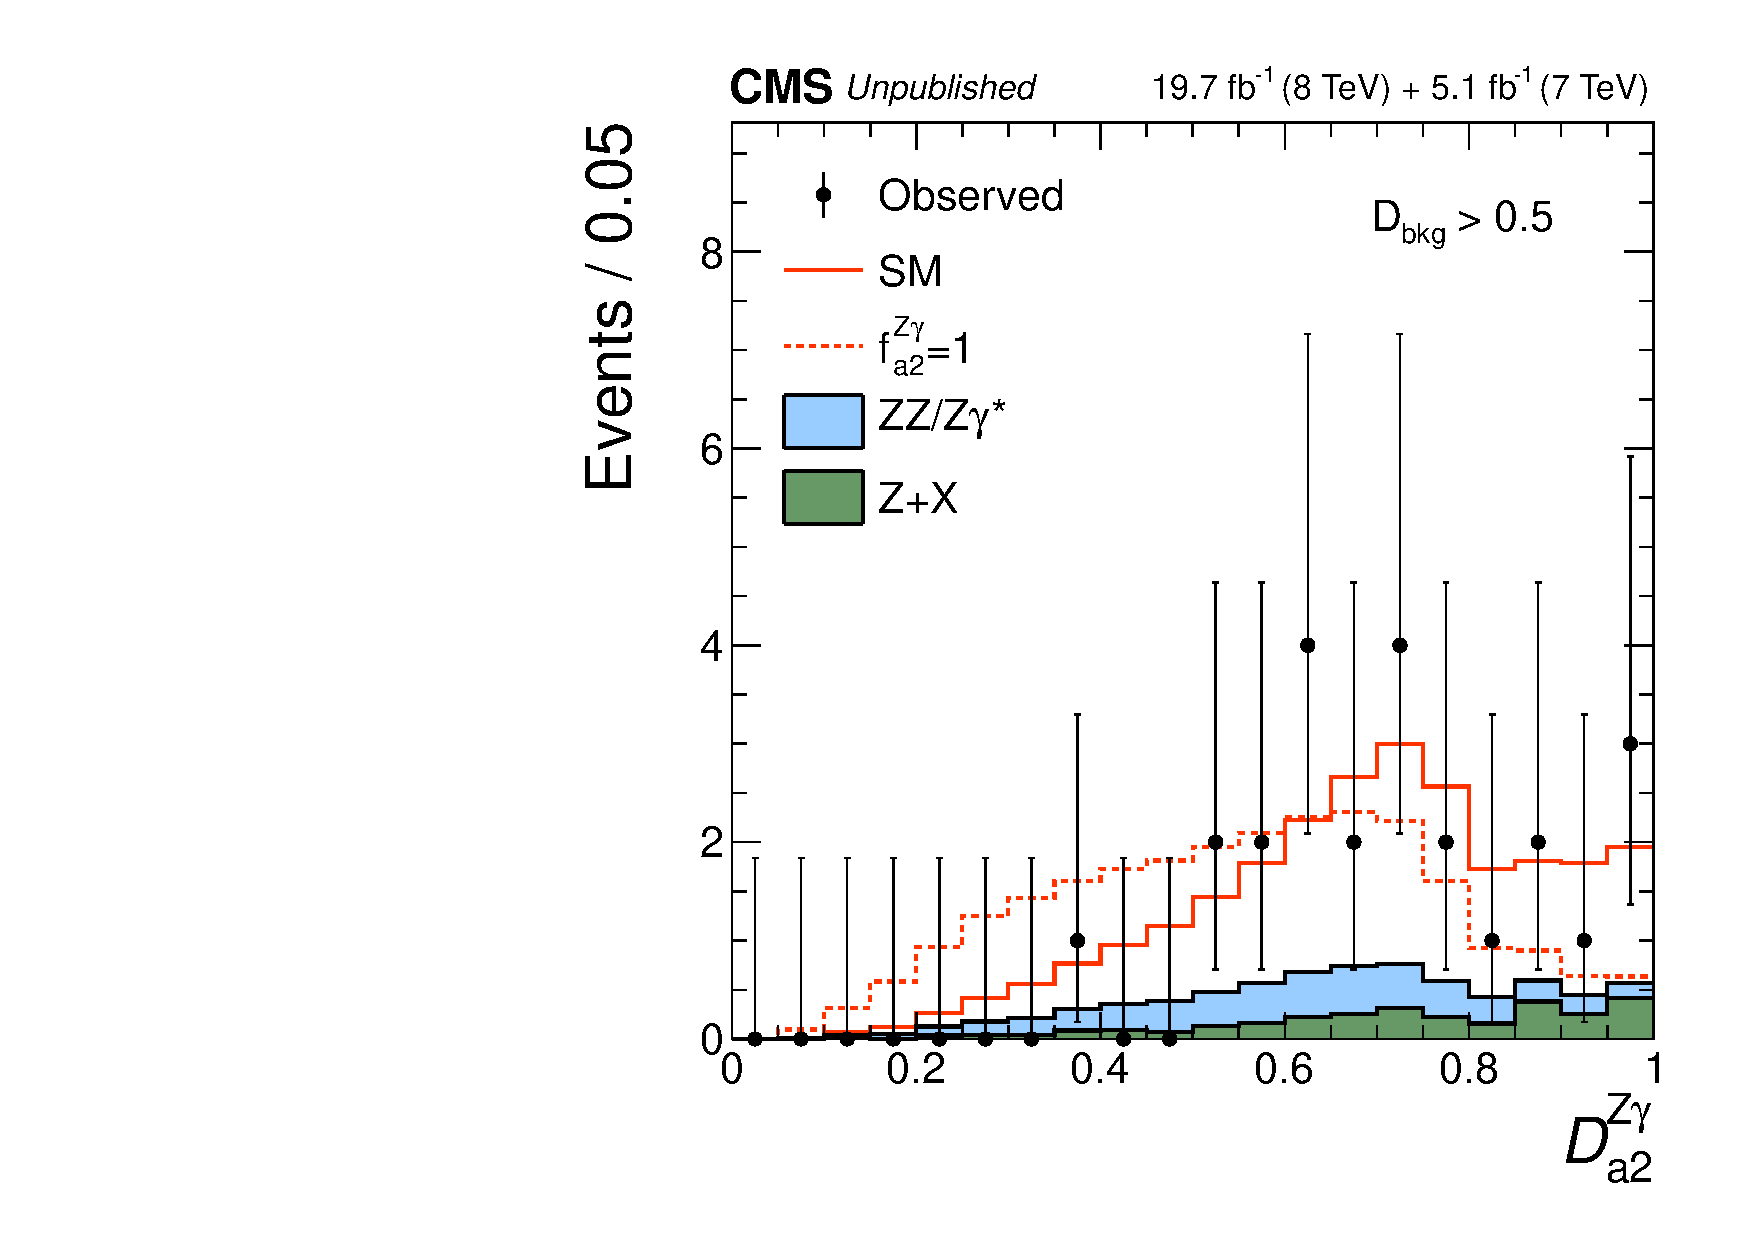
\includegraphics[width=.5\columnwidth]{HVV/Da2Zgamma}
\end{column}
\begin{column}{0.4\textwidth}
\begin{itemize}
\item discriminants for on-shell kinematics
\item all signal distributions obtained via reweighting
\end{itemize}
\end{column}
\end{columns}
\end{frame}

\begin{frame}{JHUGen in action}{ATLAS analysis $H \to ZZ^* \to 4l$\hfill [ATLAS-HIGG-2013-17] arXiv:1506.05669}
%Study of the spin and parity of the Higgs boson in diboson decays with the ATLAS detector
%http://arxiv.org/abs/1506.05669
%https://atlas.web.cern.ch/Atlas/GROUPS/PHYSICS/PAPERS/HIGG-2013-17/
\begin{columns}
\begin{column}{0.6\textwidth}
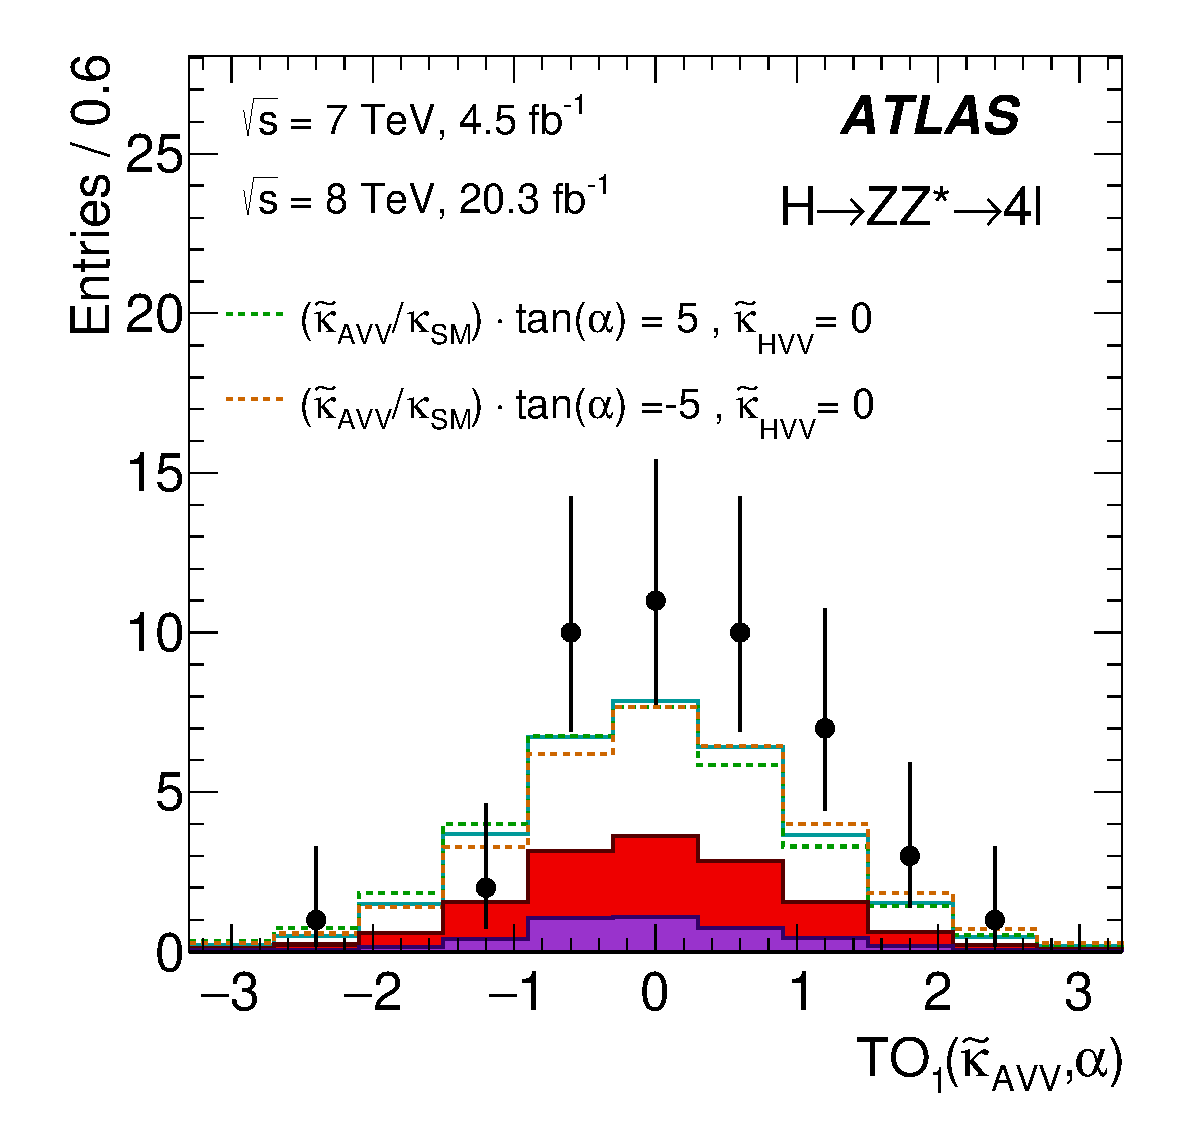
\includegraphics[width=.5\columnwidth]{ATLASHVV/TO1}
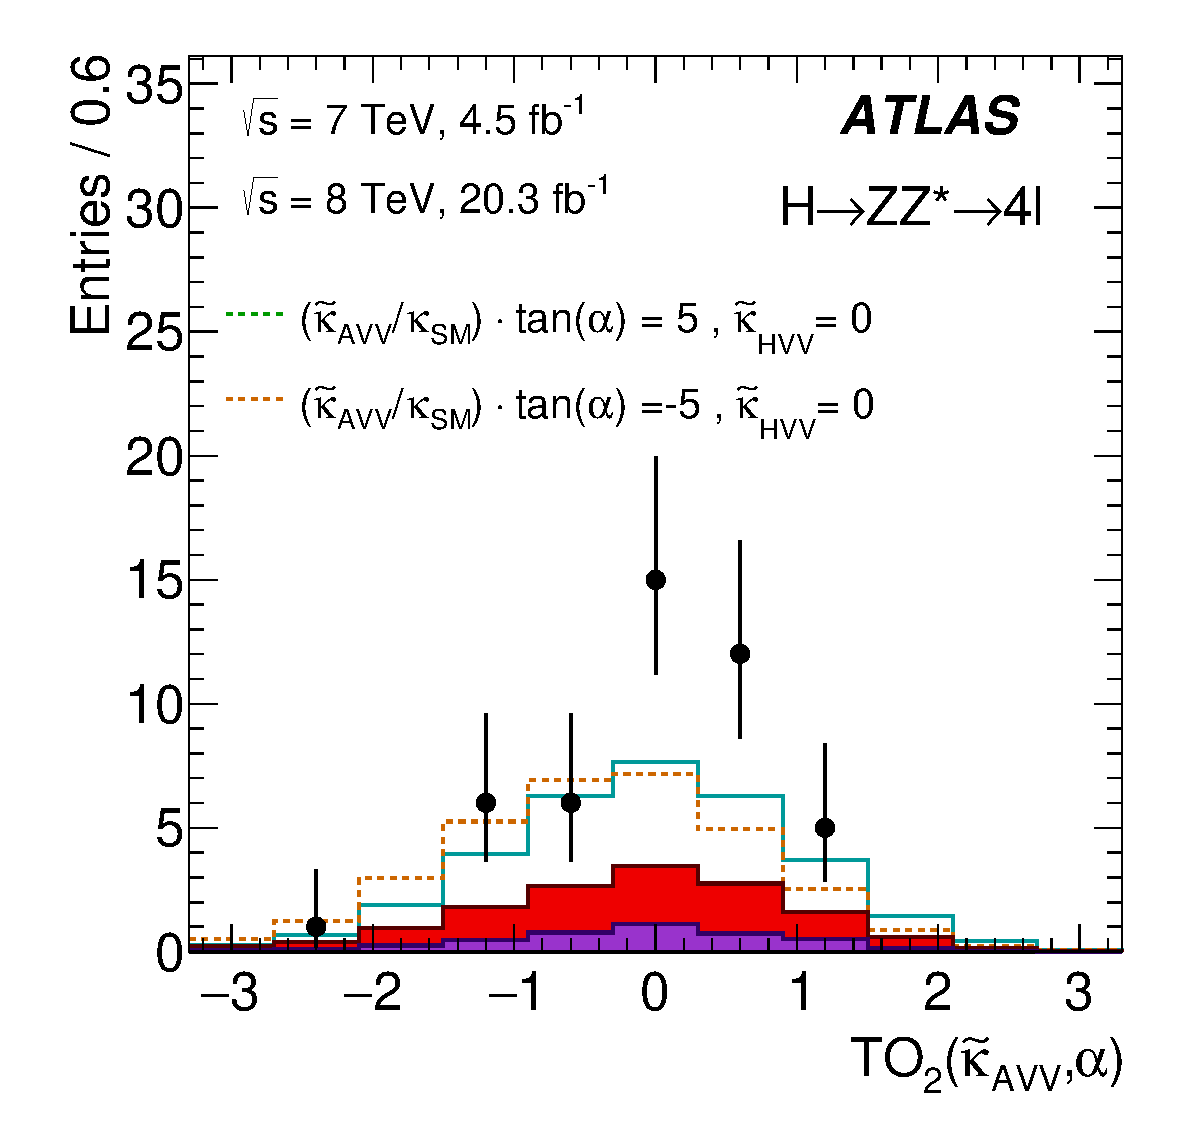
\includegraphics[width=.5\columnwidth]{ATLASHVV/TO2} \\
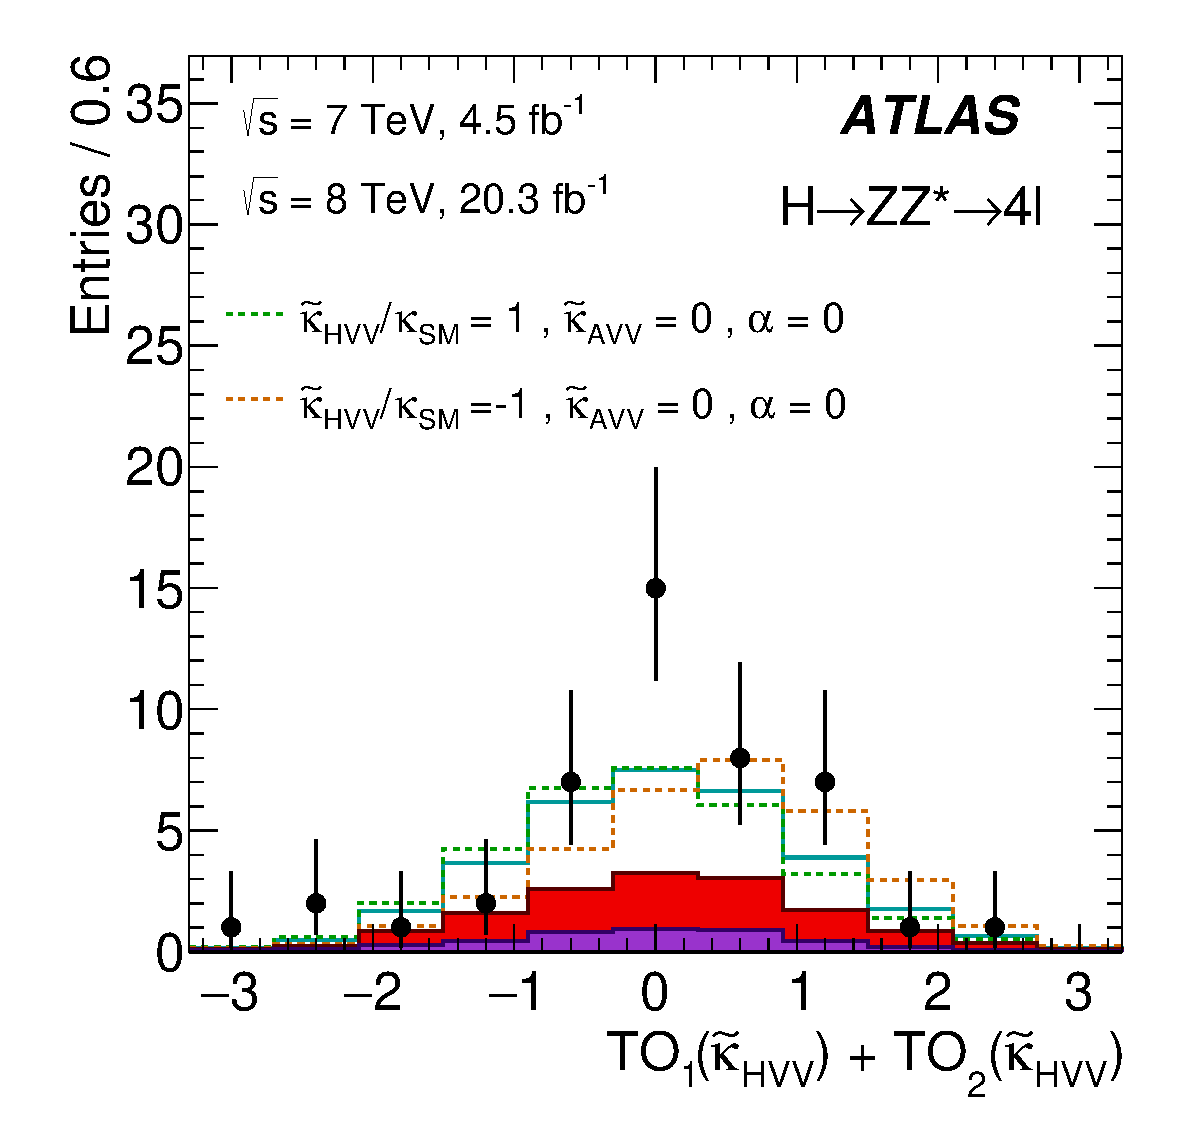
\includegraphics[width=.5\columnwidth]{ATLASHVV/TO1plusTO2}
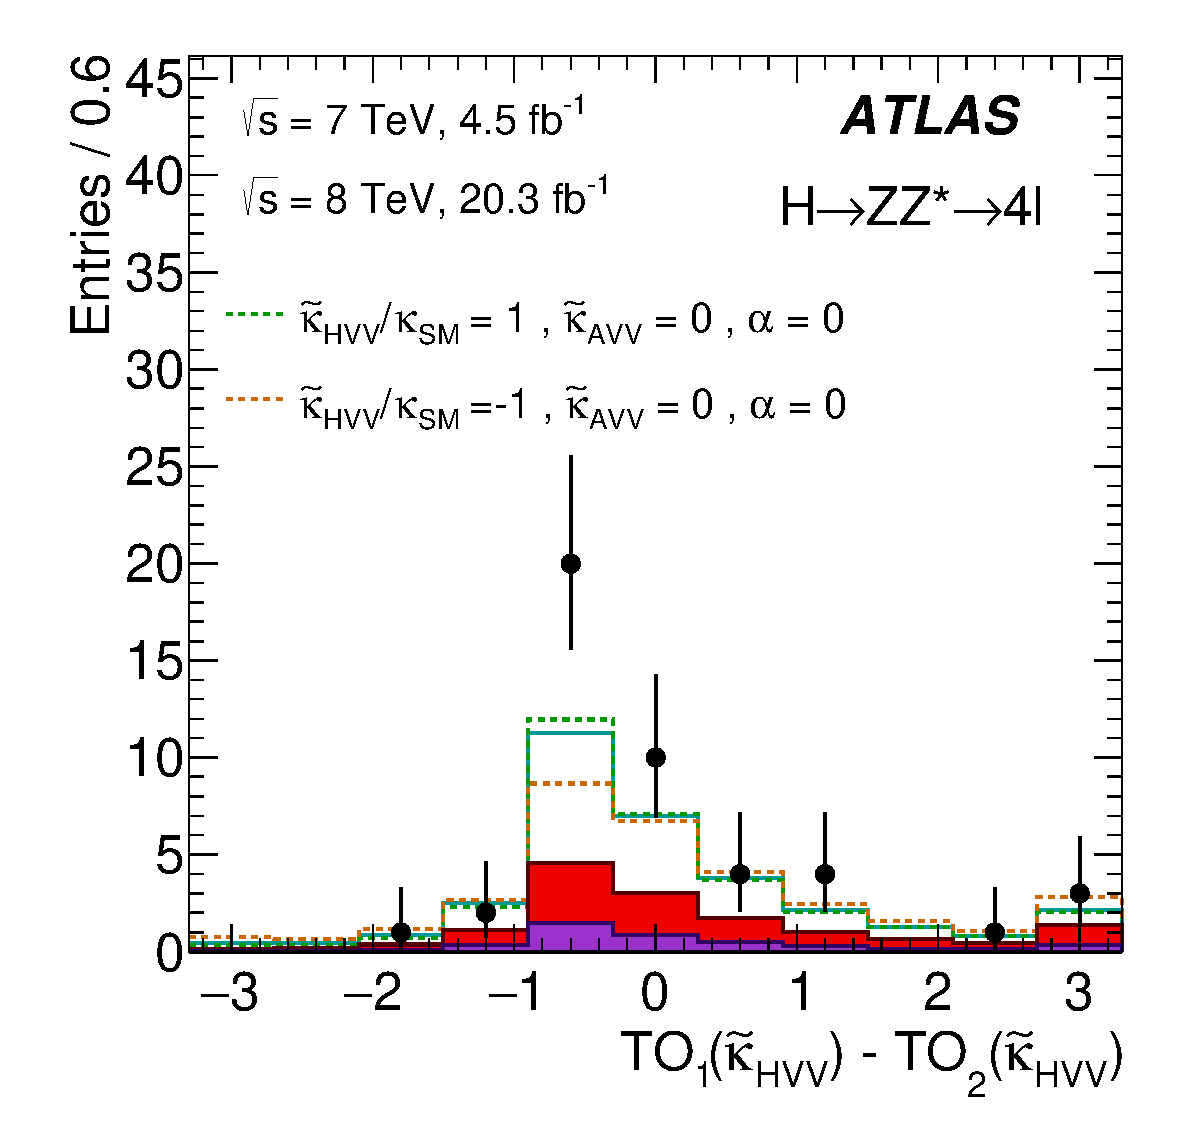
\includegraphics[width=.5\columnwidth]{ATLASHVV/TO1minusTO2}
\end{column}
\begin{column}{0.4\textwidth}
\begin{itemize}
\item Distributions of anomalous couplings were obtained by reweighting the base sample using JHUGen.
\end{itemize}
\end{column}
\end{columns}
\end{frame}

\begin{frame}{JHUGen in action}{CMS analysis $H \to WW$\hfill [CMS-HIG-14-018] arXiv:1411.3441}
\begin{columns}
\begin{column}{0.6\textwidth}
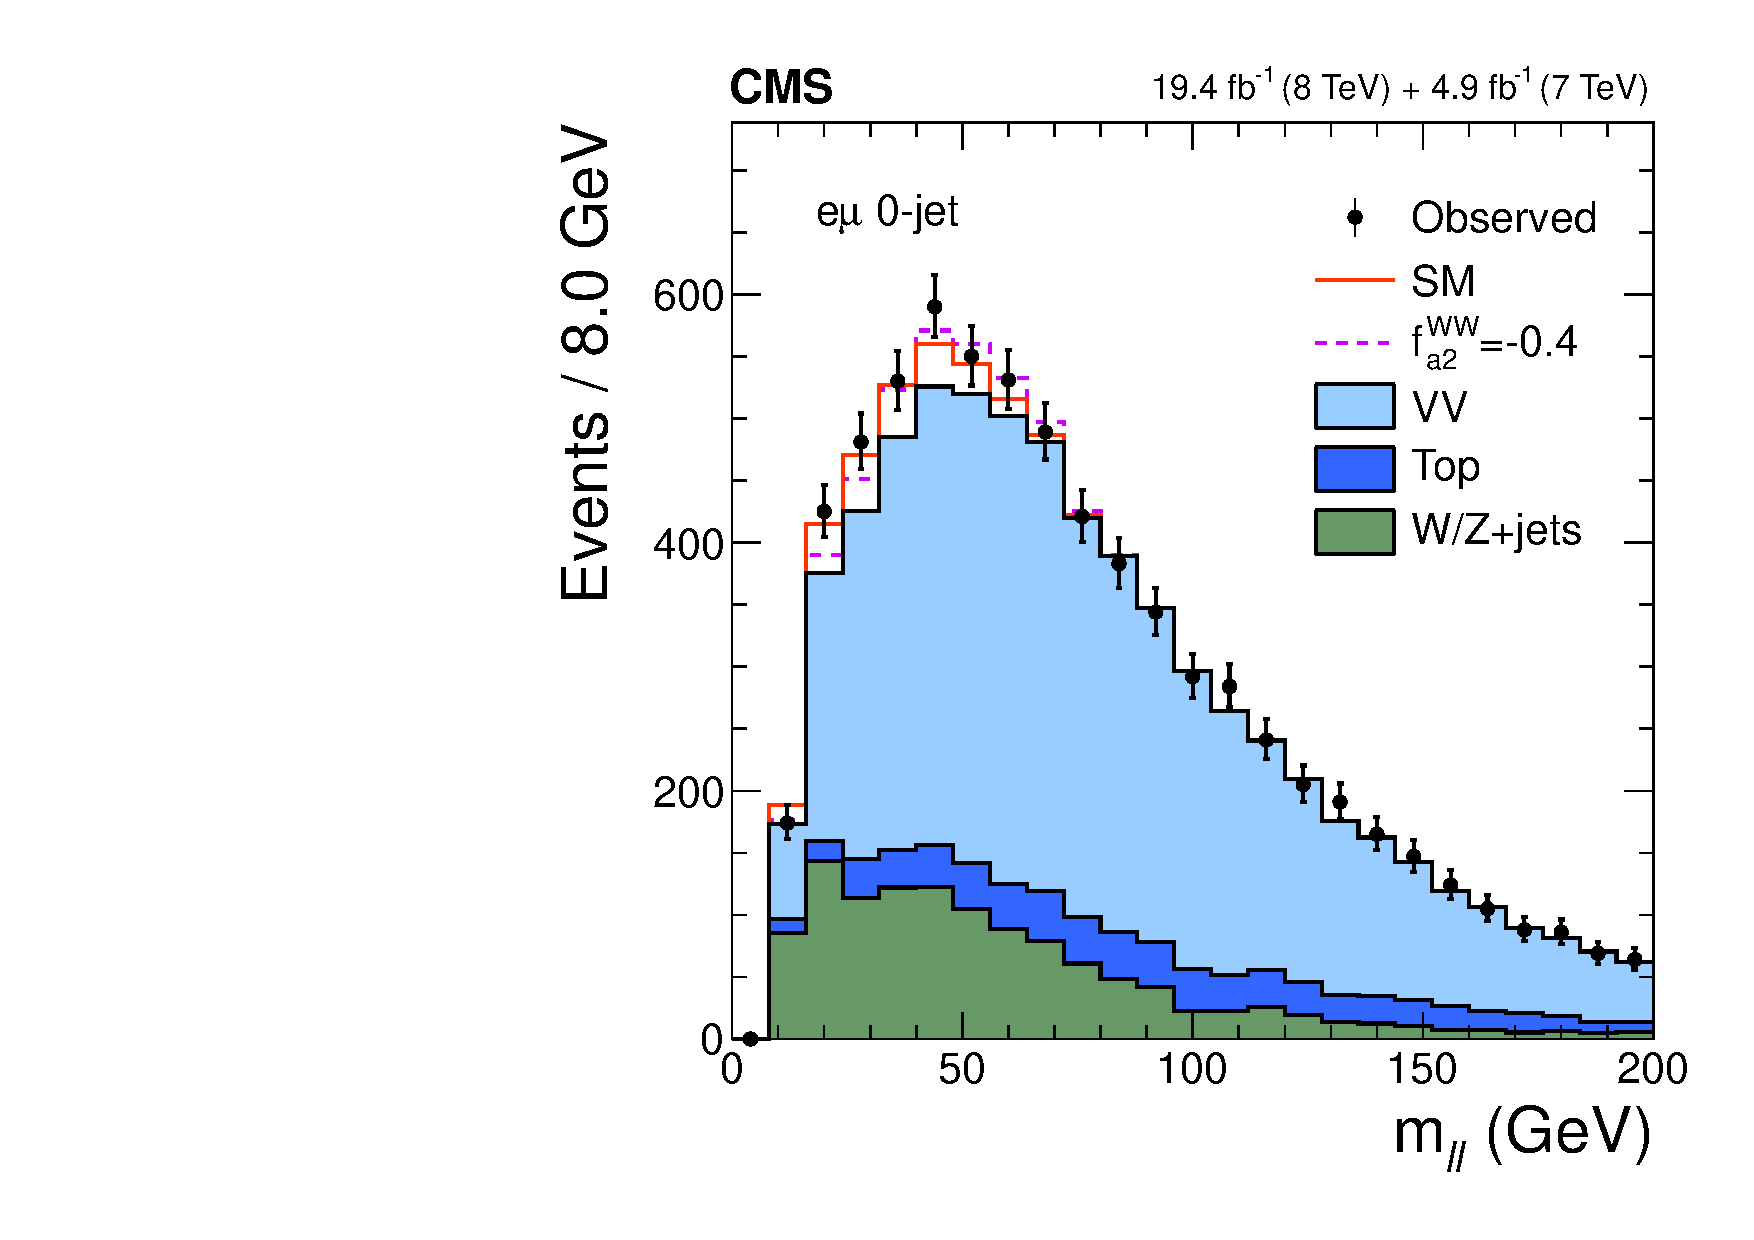
\includegraphics[width=.5\columnwidth]{HVV/WWmll}
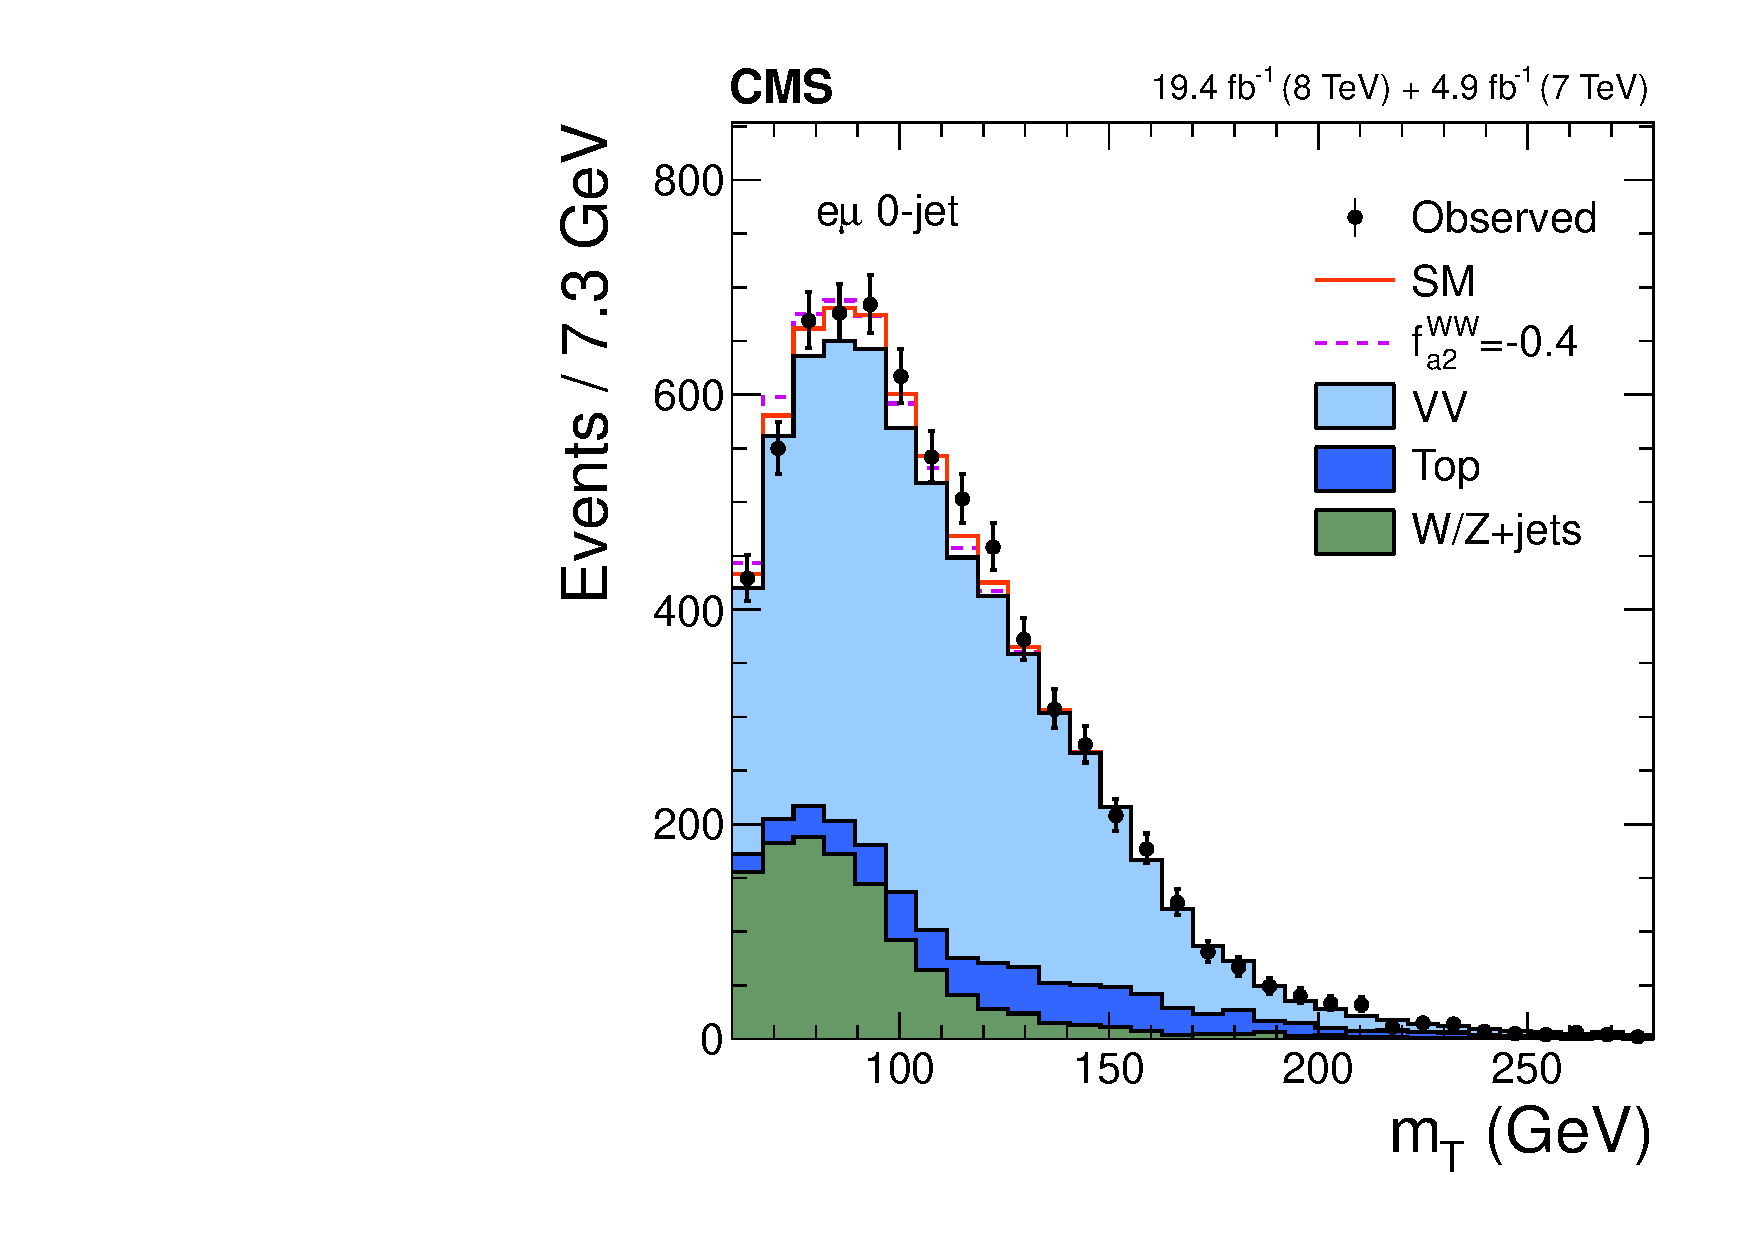
\includegraphics[width=.5\columnwidth]{HVV/WWmT} \\
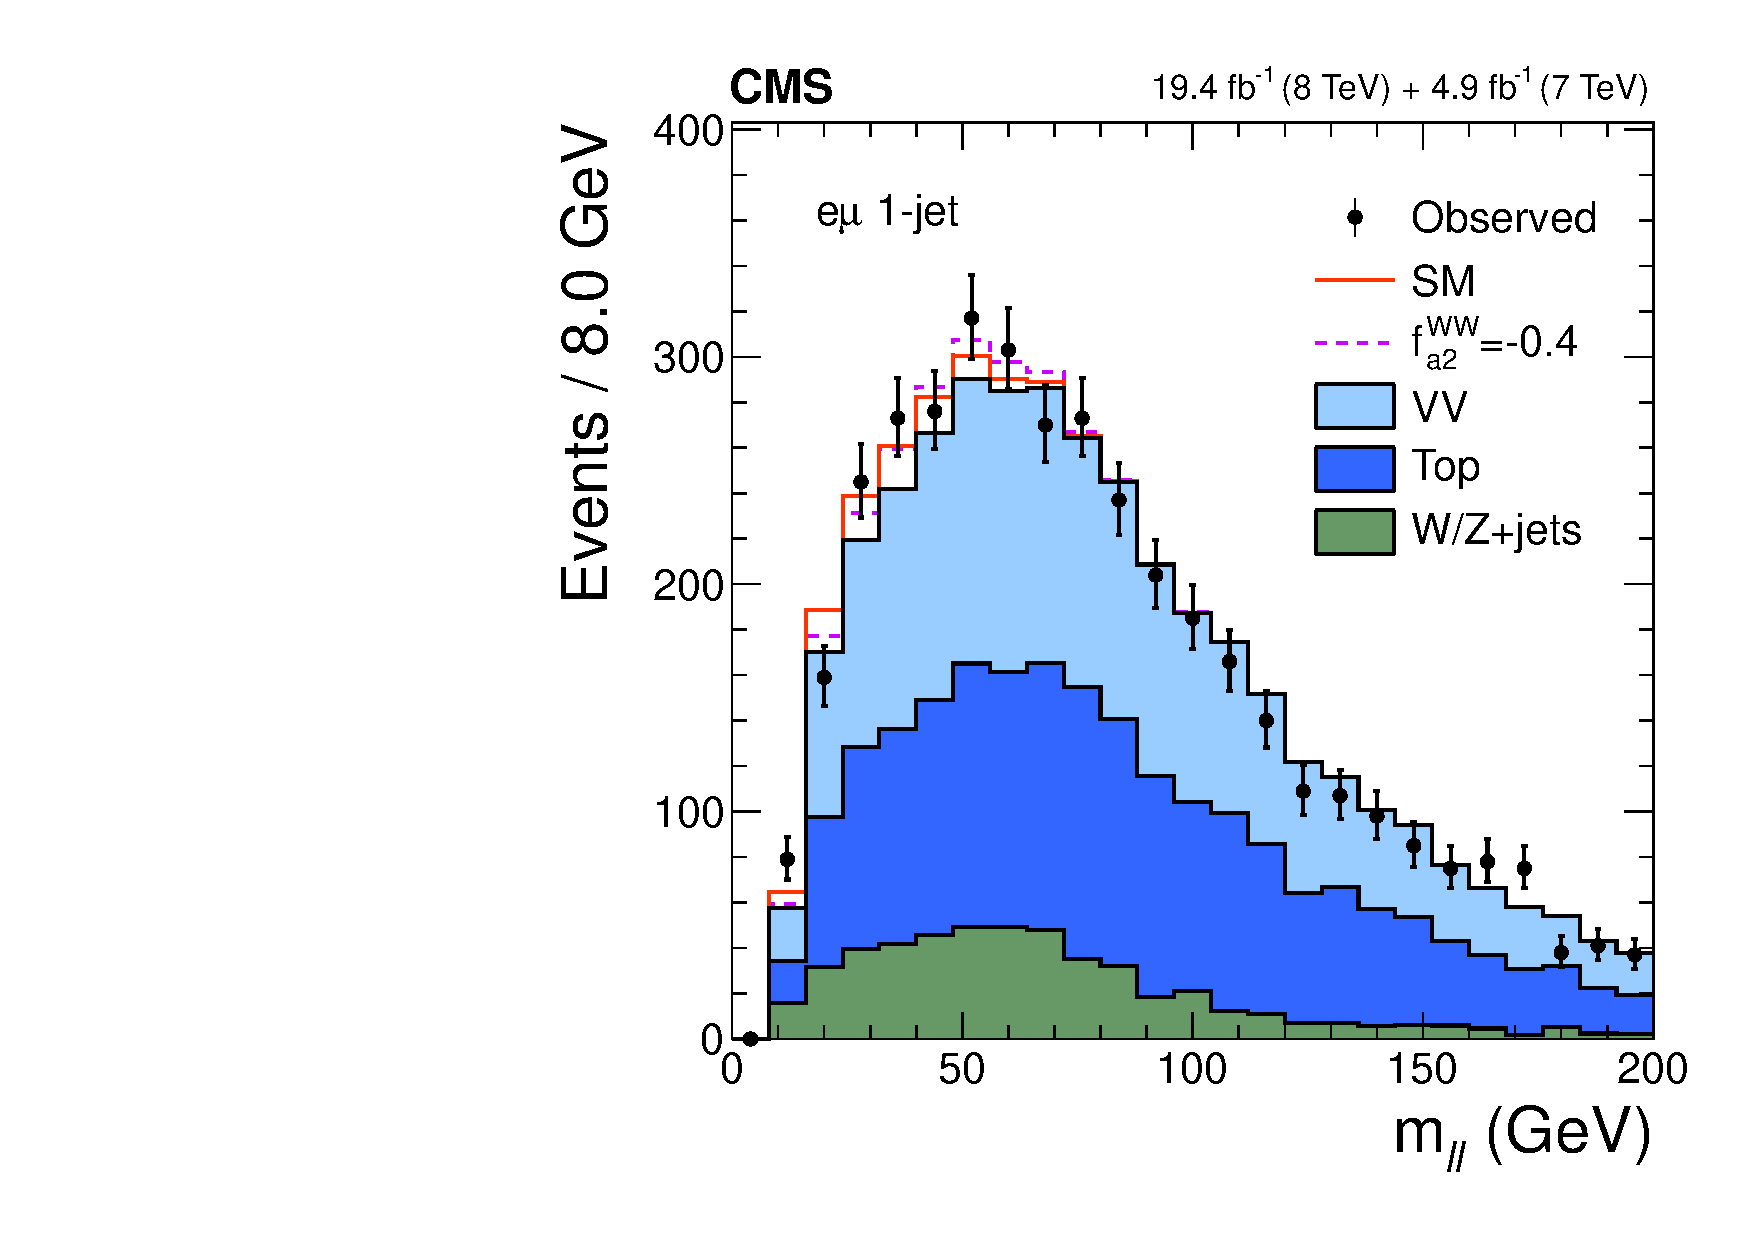
\includegraphics[width=.5\columnwidth]{HVV/WW1jetmll}
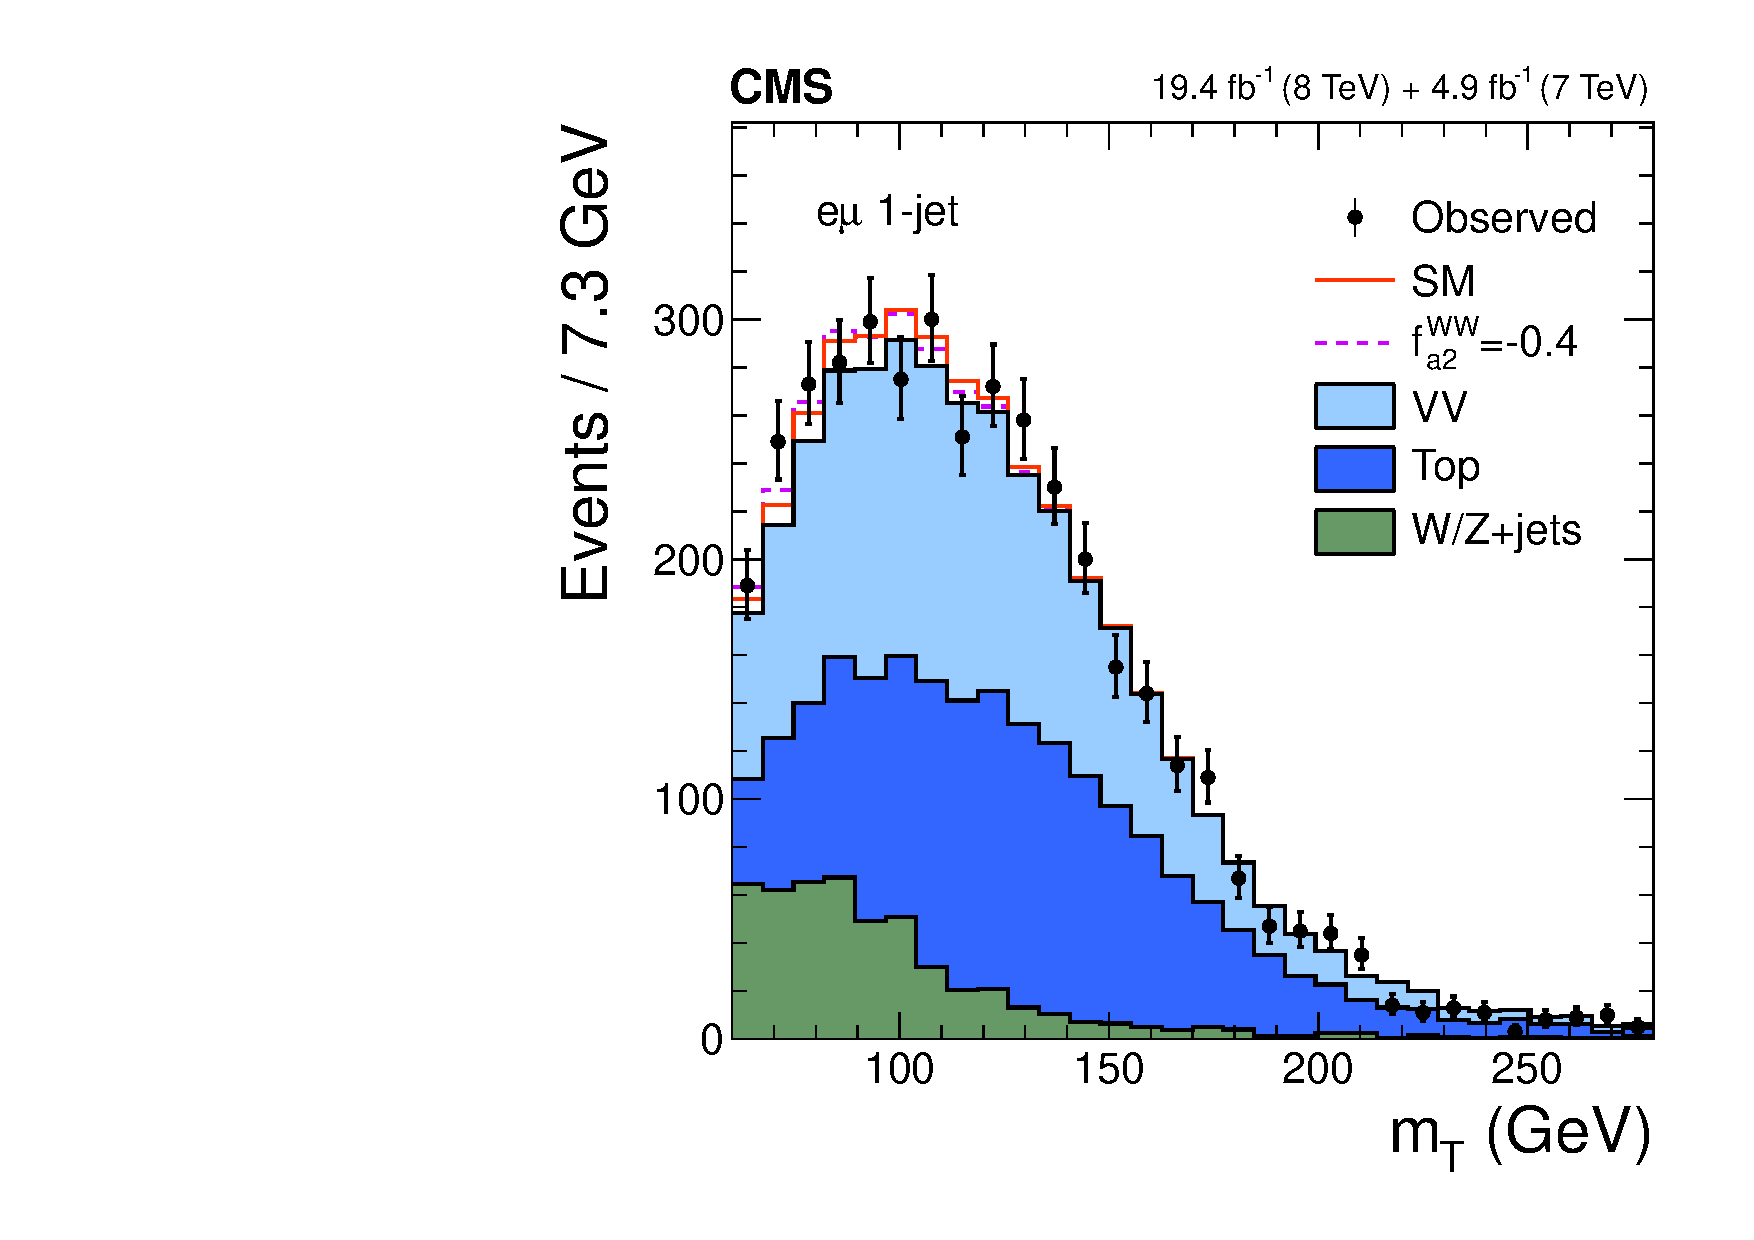
\includegraphics[width=.5\columnwidth]{HVV/WW1jetmT}
\end{column}
\begin{column}{0.4\textwidth}
\begin{itemize}
\item mass variables for on-shell kinematics
\item all signal distributions obtained via reweighting of all models to all models
\end{itemize}
\end{column}
\end{columns}
\end{frame}

\begin{frame}{JHUGen in action: Off-shell reweighting}{CMS Higgs off-shell analysis\hfill [CMS-HIG-14-036] arXiv:1507.06656}
$$\sigma^\text{on-shell}_{vv\to H\to ZZ}\sim\mu_{vvH}\therefore \sigma^\text{off-shell}_{vv\to H\to ZZ}\sim \mu_{vvH}\times\Gamma_H$$
\begin{columns}
\begin{column}{0.1\textwidth}
Gluon fusion signal only % (to be replaced with non Work in Progress from Ulascan)
\end{column}
\begin{column}{0.75\textwidth}
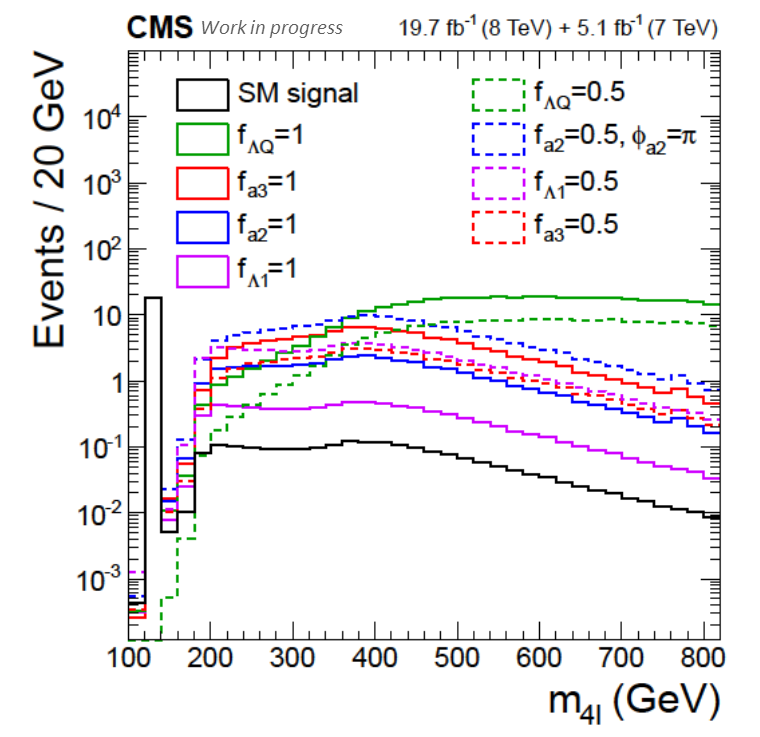
\includegraphics[width=0.5\columnwidth]{lifetime/signalonly}
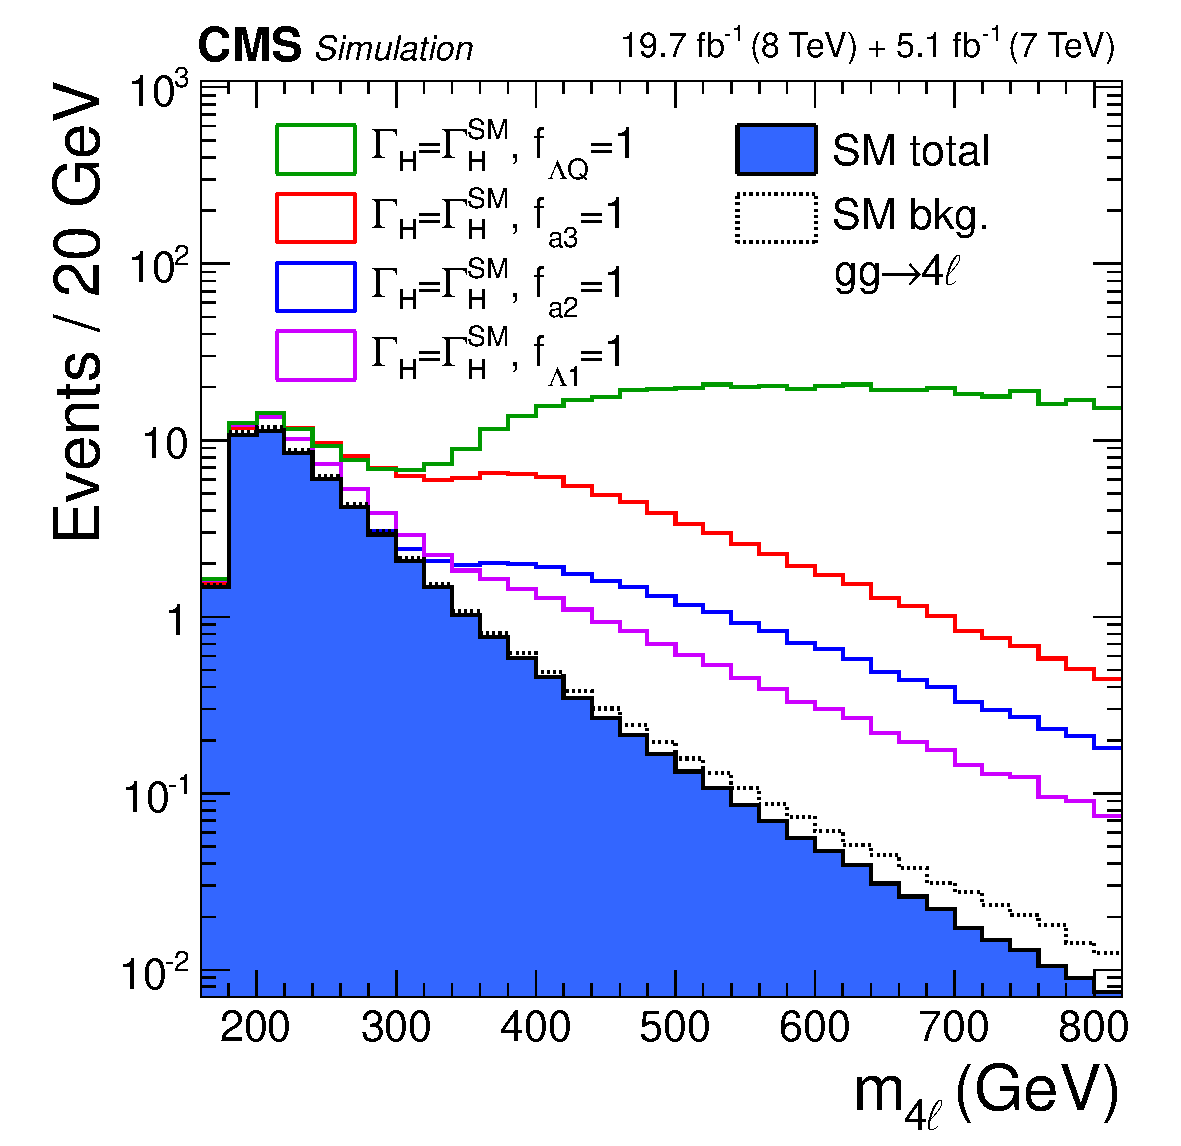
\includegraphics[width=0.5\columnwidth]{lifetime/fig1}
\end{column}
\begin{column}{0.15\textwidth}
Gluon fusion signal + bkg. + int.
\end{column}
\end{columns}
\begin{itemize} \footnotesize
\item all signal distributions obtained via re-weighting
\item use add-on for MCFM to implement anomalous couplings and interface MELA with MCFM to include signal + background + interference
\end{itemize}
\end{frame}

\begin{frame}{JHUGen in action: Background reweighting}{H. Roskes, \emph{Validation of the Higgs boson spin-parity
analysis with $Z\to 4l$ data}\\ \url{http://meetings.aps.org/link/BAPS.2015.APR.X16.8}}
\begin{columns}
\begin{column}{0.55\textwidth}
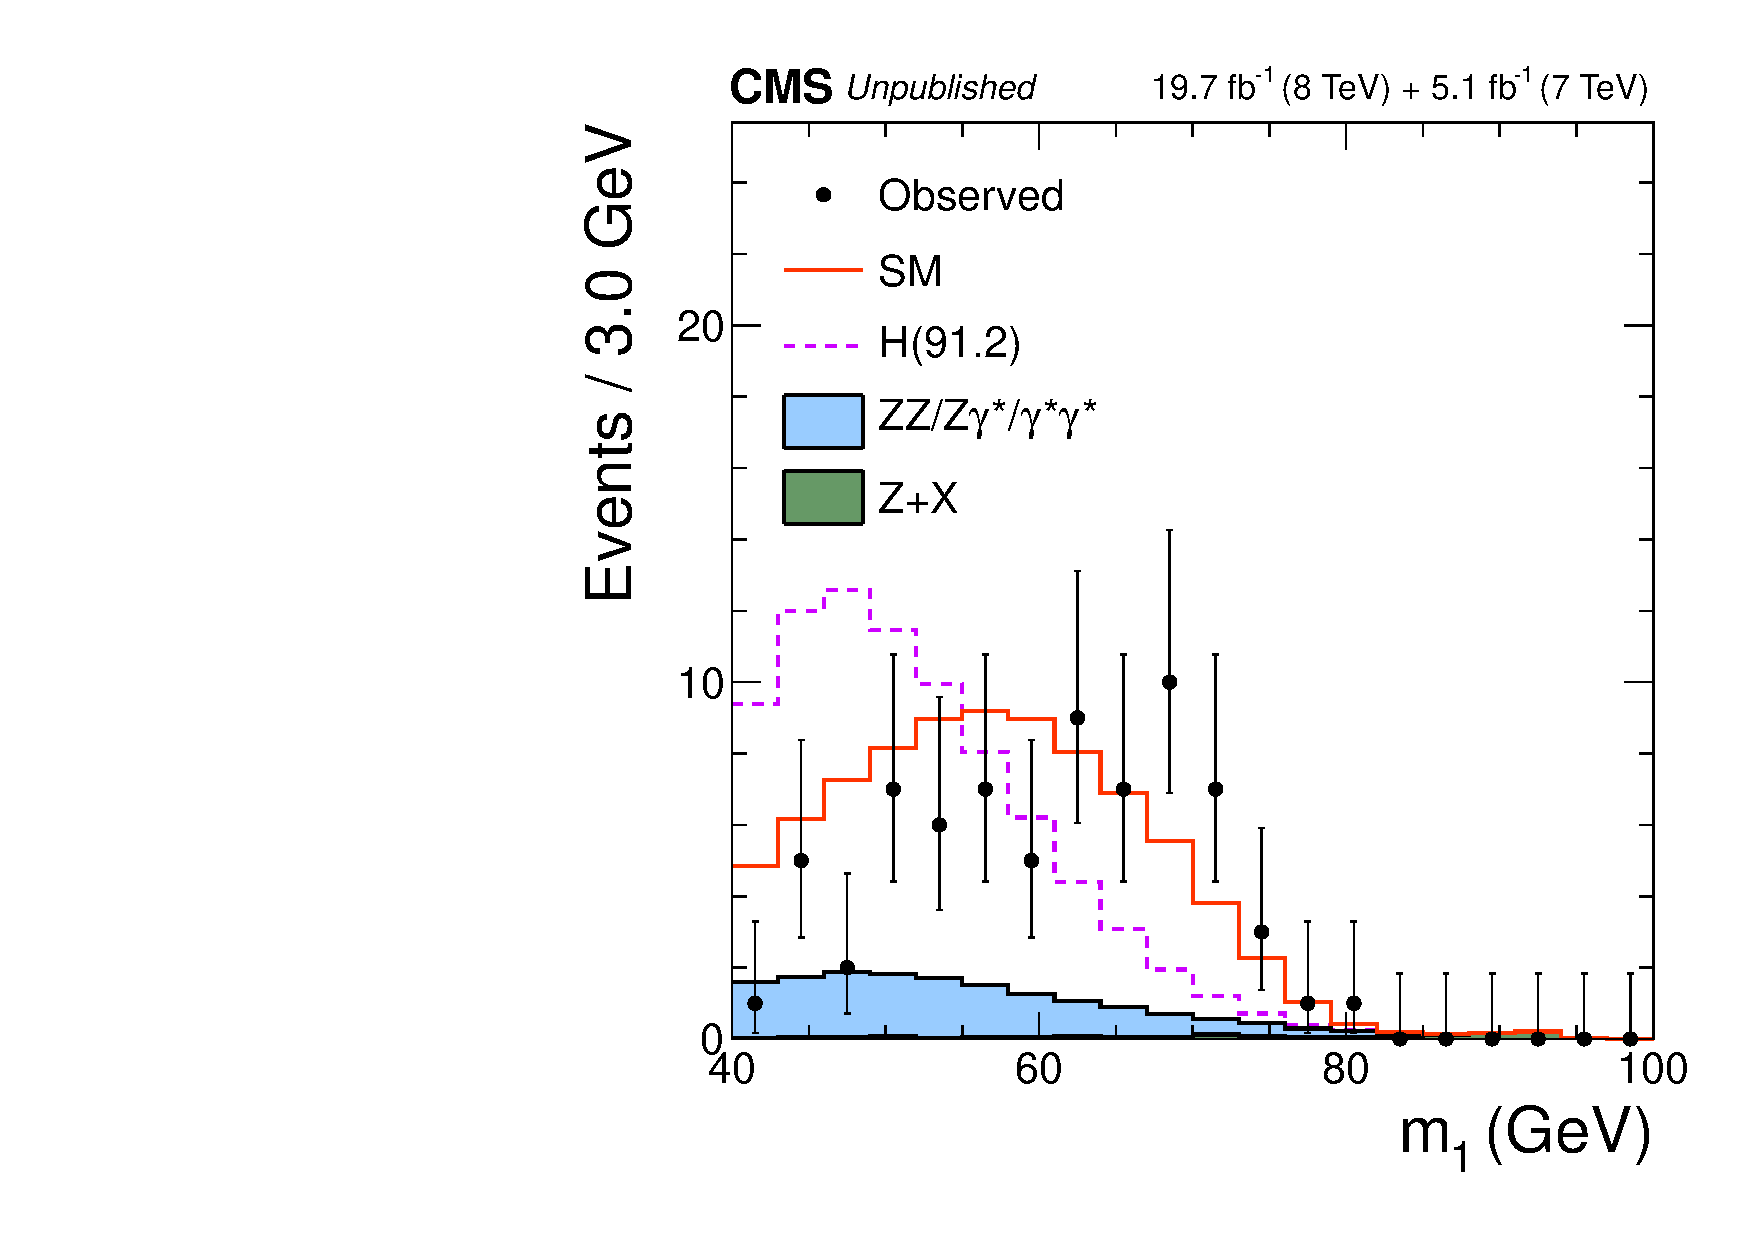
\includegraphics[width=.5\columnwidth]{HVV/Z4lm1}
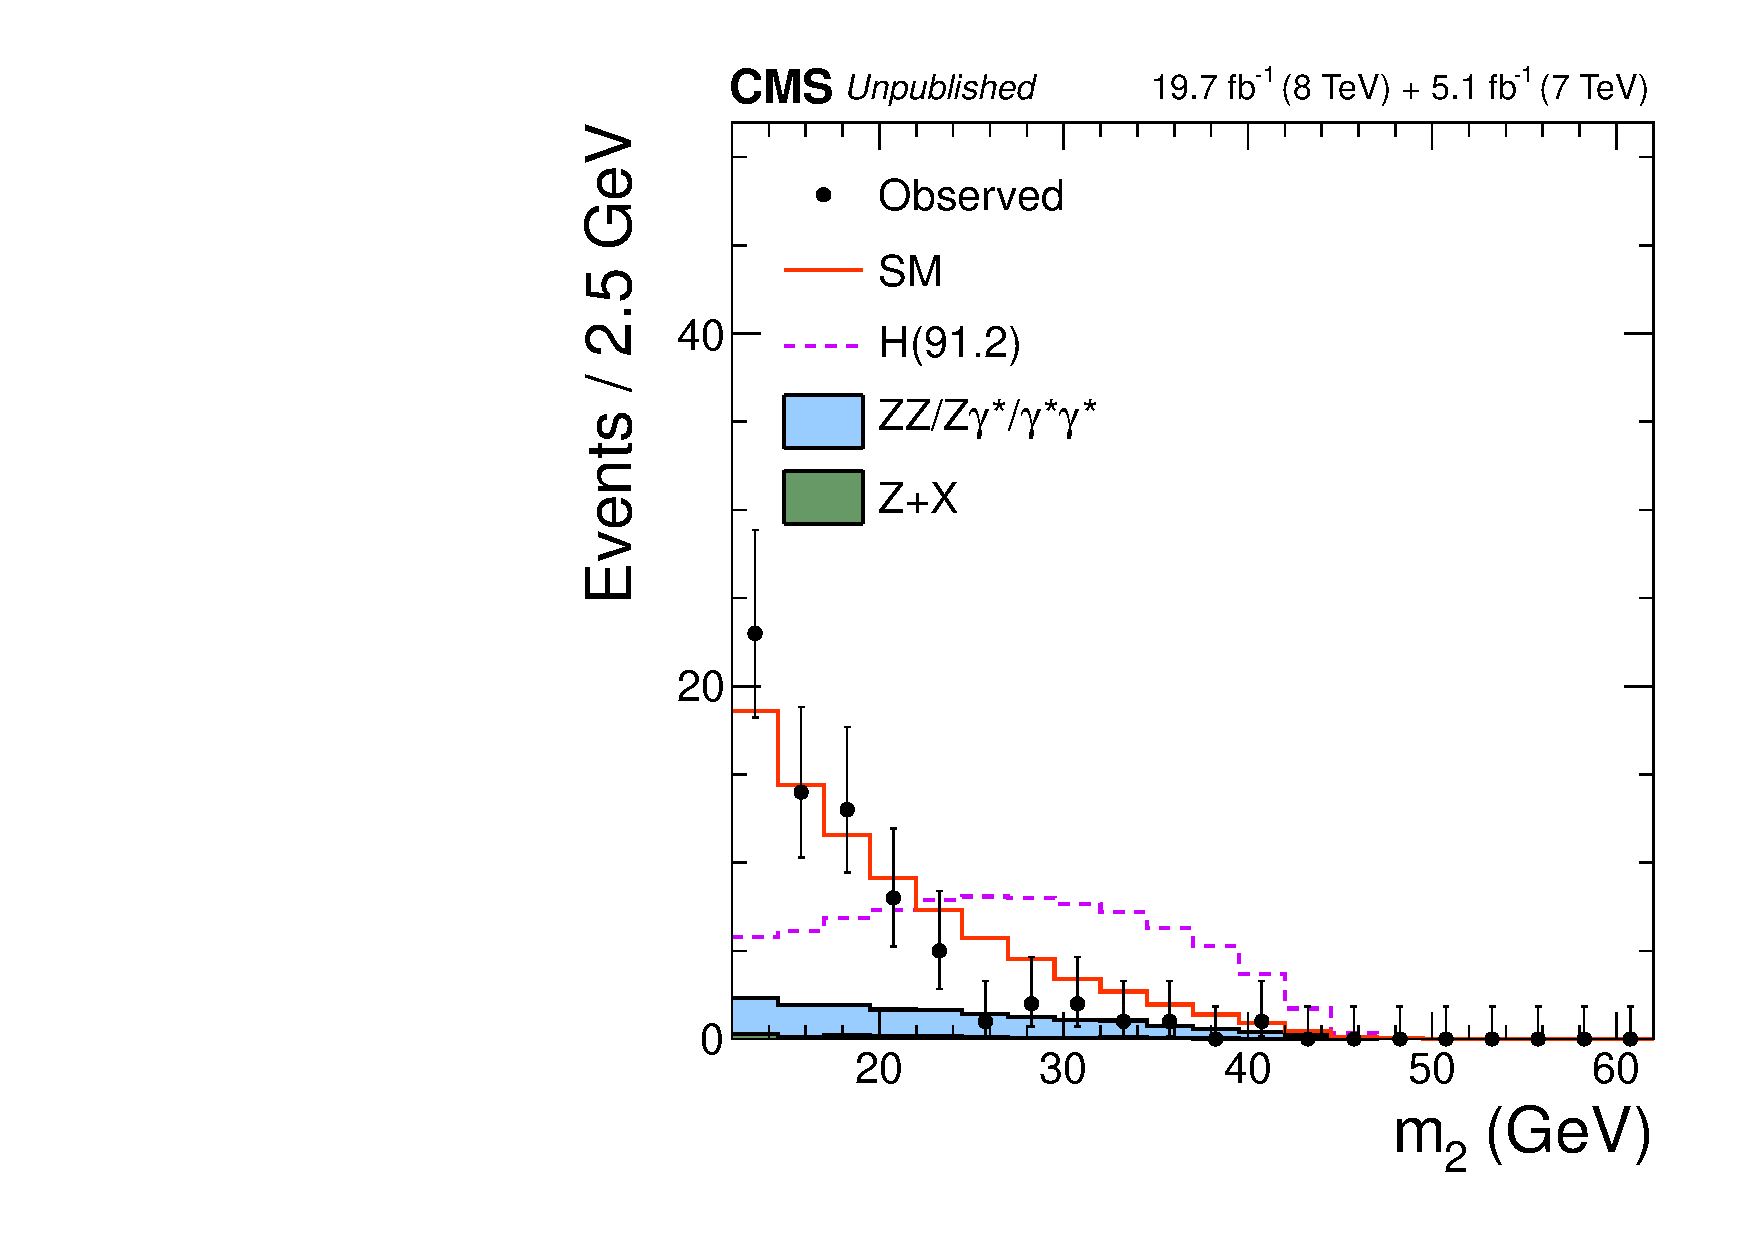
\includegraphics[width=.5\columnwidth]{HVV/Z4lm2} \\
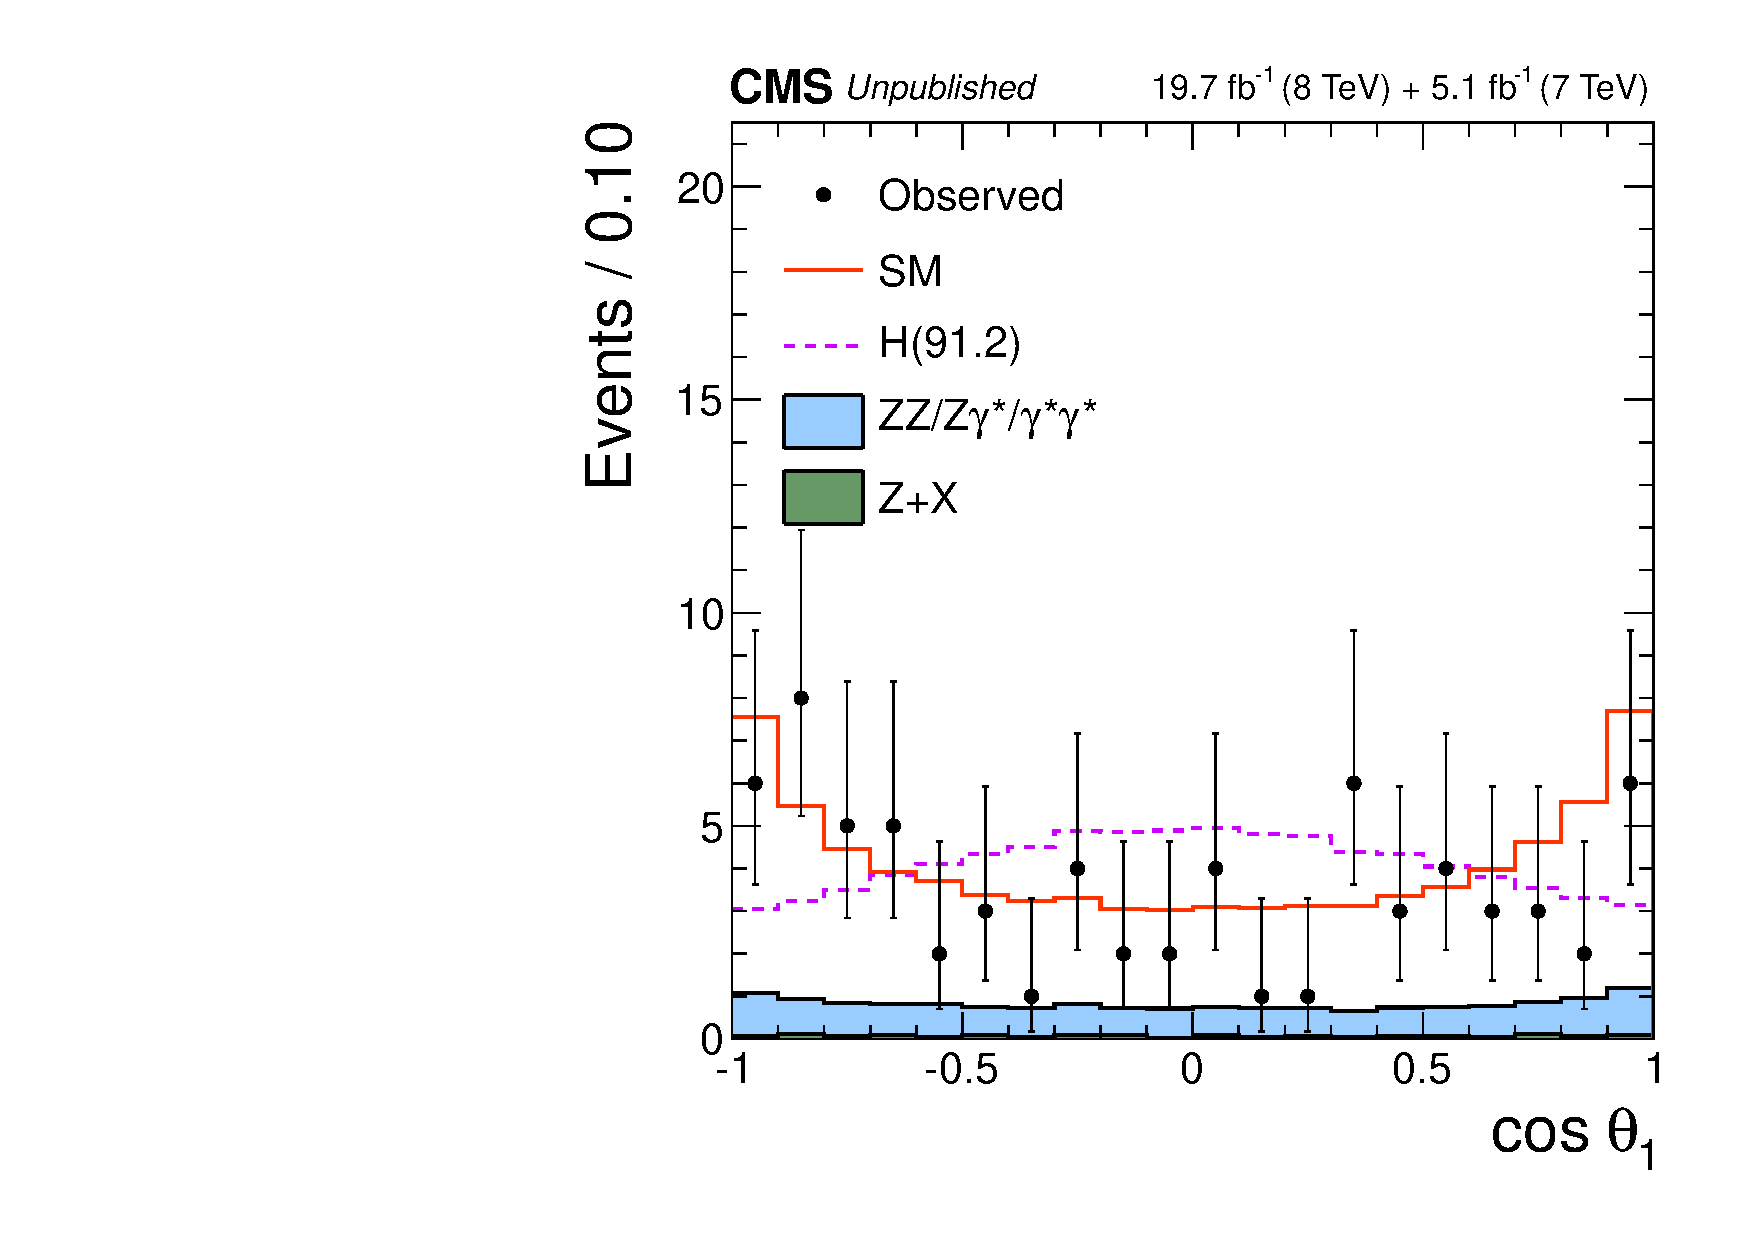
\includegraphics[width=.5\columnwidth]{HVV/Z4lcostheta1}
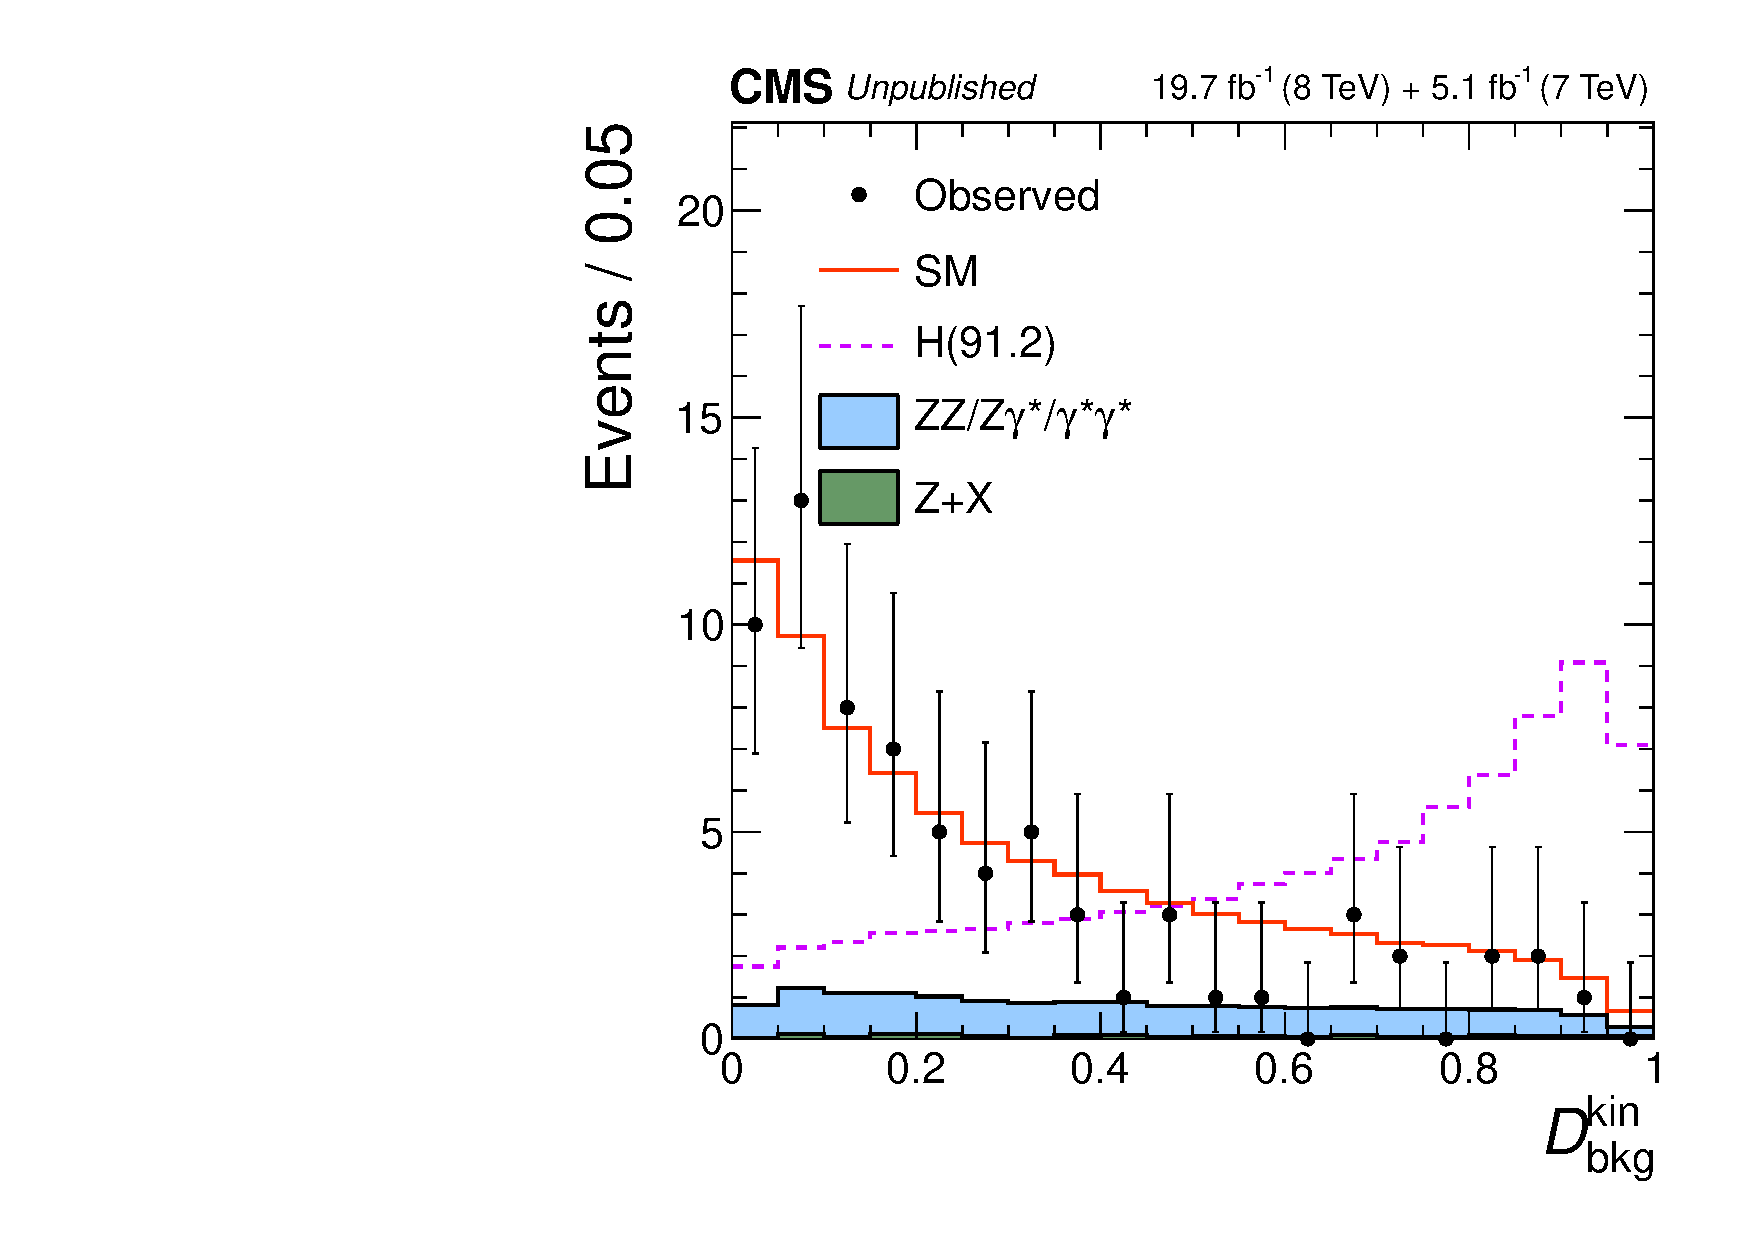
\includegraphics[width=.5\columnwidth]{HVV/Z4lDbkgkin}
\end{column}
\begin{column}{0.45\textwidth}
\begin{itemize}
\item Mixture of $s$, $t$, and $u$ channels generated with POWHEG
\item MELA reweighting used $s$ and $t+u$ channels separately, along with interference
\item $gg$ background is obtained by reweighting $q\bar{q}$
\end{itemize}
\end{column}
\end{columns}
\end{frame}

\begin{frame}{$ttH$}
Study top quarks produced in association with Higgs
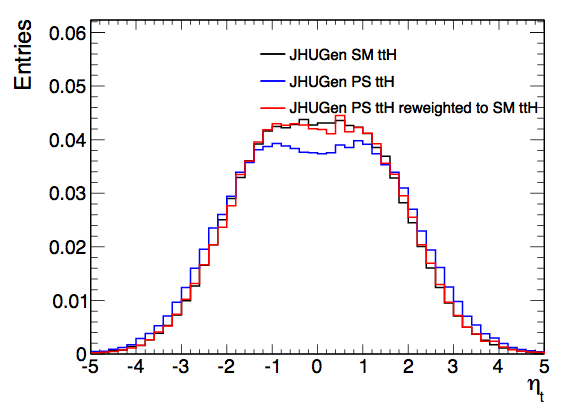
\includegraphics[width=.5\textwidth]{ttH/etatop}
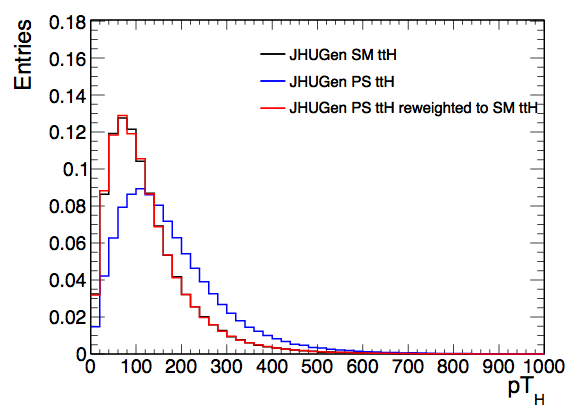
\includegraphics[width=.5\textwidth]{ttH/pTH}
\begin{itemize}
\item Associated top production is very sensitive to the incoming partons
\begin{itemize}[label=$\Rightarrow$]
\item Include PDF in MELA weight
\[
\sim f^p_i\left(x_1\right)f^p_j\left(x_2\right)\times\left|\mathcal{M}\left(d\Pi\right)\right|^2
\]
\end{itemize}
\item Similar for VBF, VH, $H+j\left(j\right)$
\end{itemize}
\end{frame}

\begin{frame}{Summary}
\begin{itemize}
\item JHUGen is a flexible framework for studies of anomalous couplings in spin-0,1,2 resonance production and other associated production modes.
\begin{multicols}{2}
\begin{itemize}
\item VBF
\item $H+$1 or 2 QCD jets
\item $VH$
\item $t\bar{t}H$
\item More to come
\item %blank for alignment
\end{itemize}
\end{multicols}
\item JHUGenMELA provides respective matrix elements for:
\begin{itemize}
\item optimal discriminants for anomalous coupling fits
\item background suppression
\item re-weighting
\end{itemize}
\item Fruitful application in various analyses by CMS and ATLAS
\item Future developments:
\begin{itemize}
\item Application to more Higgs production mechanisms and decay channels
\end{itemize}
\end{itemize}
\end{frame}
\end{document}
